\documentclass[aspectratio=169, 10pt, professionalfonts]{beamer}

% =============================================================================
%  Beamer configuration -- modernized for thesis defense
% =============================================================================

\usepackage[utf8]{inputenc}
\usepackage[T1]{fontenc}
\usepackage[english]{babel}

\mode<presentation> {
    \usetheme{Montpellier}
    % We override the color theme below with a custom palette
}

% -----------------------------------------------------------------------------
%  Modern color palette (Tec de Monterrey inspired)
% -----------------------------------------------------------------------------
\definecolor{tecblue}{HTML}{0033A0}
\definecolor{tecdark}{HTML}{00205B}
\definecolor{tecaccent}{HTML}{D52B1E}
\definecolor{tecorange}{HTML}{F39200}
\definecolor{tecgreen}{HTML}{2E8B57}
\definecolor{slidegray}{HTML}{4A4A4A}
\definecolor{slidelight}{HTML}{F5F7FA}

\setbeamercolor{structure}{fg=tecblue}
\setbeamercolor{alerted text}{fg=tecaccent}
\setbeamercolor{title}{fg=tecdark}
\setbeamercolor{frametitle}{fg=tecdark}
\setbeamercolor{block title}{bg=tecblue!15,fg=tecdark}
\setbeamercolor{block body}{bg=tecblue!5,fg=slidegray}
\setbeamercolor{block title alerted}{bg=tecaccent!15,fg=tecaccent}
\setbeamercolor{block body alerted}{bg=tecaccent!5,fg=slidegray}
\setbeamercolor{block title example}{bg=tecgreen!15,fg=tecgreen}
\setbeamercolor{block body example}{bg=tecgreen!5,fg=slidegray}
\setbeamercolor{itemize item}{fg=tecblue}
\setbeamercolor{itemize subitem}{fg=tecblue!70}
\setbeamercolor{enumerate item}{fg=tecblue}
\setbeamercolor{section in toc}{fg=tecdark}
\setbeamercolor{subsection in toc}{fg=slidegray}

% Slightly bolder fonts for titles
\setbeamerfont{frametitle}{series=\bfseries,size=\large}
\setbeamerfont{title}{series=\bfseries}
\setbeamerfont{block title}{series=\bfseries}

% -----------------------------------------------------------------------------
%  Header / footer
% -----------------------------------------------------------------------------
\addtobeamertemplate{headline}{}{%
\begin{tikzpicture}[remember picture,overlay]
\node at([shift={(0.4\paperwidth,-0.53)}]current page.north) {%

\includegraphics[height=0.7cm,width=2.67cm]{./DATA/ICON/LogoHead.pdf}};
\end{tikzpicture}}

% -----------------------------------------------------------------------------
%  Packages
% -----------------------------------------------------------------------------
\usepackage{graphicx}
\usepackage{booktabs}
\usepackage{ragged2e}
\usepackage[justification=justified,format=plain]{caption}
\usepackage{amsmath,amssymb,mathtools,relsize}
\usepackage{multirow}
\usepackage{subcaption}
\usepackage{multicol}
\usepackage{datetime}
\usepackage{listings}
\usepackage{overpic}
\usepackage{makecell}
\usepackage{algorithm,algorithmic}
\usepackage{tikz}
\usepackage{colortbl}
\usepackage{marvosym}
\usepackage{xcolor}
\usepackage{array}

\hypersetup{colorlinks,
    citecolor=tecblue,
    linkcolor=tecblue,
    urlcolor=tecblue,
    filecolor=tecaccent,
    bookmarksopenlevel=4
}

% -----------------------------------------------------------------------------
%  Code listings
% -----------------------------------------------------------------------------
\definecolor{codegreen}{rgb}{0,0.6,0}
\definecolor{codegray}{rgb}{0.5,0.5,0.5}
\definecolor{codepurple}{rgb}{0.58,0,0.82}
\definecolor{backcolour}{rgb}{0.95,0.95,0.92}

\lstdefinestyle{mystyle}{
    backgroundcolor=\color{backcolour},
    commentstyle=\color{codegreen},
    keywordstyle=\color{magenta},
    numberstyle=\tiny\color{codegray},
    stringstyle=\color{codepurple},
    basicstyle=\ttfamily\footnotesize,
    breakatwhitespace=false,
    breaklines=true,
    captionpos=b,
    keepspaces=true,
    numbers=left,
    numbersep=5pt,
    showspaces=false,
    showstringspaces=false,
    showtabs=false,
    tabsize=2
}
\lstset{style=mystyle}

% -----------------------------------------------------------------------------
%  tcolorbox-based note boxes
% -----------------------------------------------------------------------------
\usepackage[most]{tcolorbox}
\tcbuselibrary{skins,xparse,listings}

\tcbset{textmarker/.style={%
    enhanced,
    parbox=false,boxrule=0mm,boxsep=0mm,arc=0mm,
    outer arc=0mm,left=6mm,right=3mm,top=7pt,bottom=7pt,
    toptitle=1mm,bottomtitle=1mm,oversize}}

\newtcolorbox{hintBox}{textmarker,
    borderline west={6pt}{0pt}{tecorange},
    colback=tecorange!10!white}
\newtcolorbox{importantBox}{textmarker,
    borderline west={6pt}{0pt}{tecaccent},
    colback=tecaccent!10!white}
\newtcolorbox{noteBox}{textmarker,
    borderline west={6pt}{0pt}{tecgreen},
    colback=tecgreen!10!white}
\newtcolorbox{infoBox}{textmarker,
    borderline west={6pt}{0pt}{tecblue},
    colback=tecblue!8!white}

\newcommand{\greennote}[1]{\begin{noteBox} \textbf{Note:} #1 \end{noteBox}}
\newcommand{\yellownote}[1]{\begin{hintBox} \textbf{Hint:} #1 \end{hintBox}}
\newcommand{\rednote}[1]{\begin{importantBox} \textbf{Important:} #1 \end{importantBox}}
\newcommand{\bluenote}[1]{\begin{infoBox} \textbf{Info:} #1 \end{infoBox}}

% -----------------------------------------------------------------------------
%  Math operators
% -----------------------------------------------------------------------------
\DeclareMathOperator*{\argmax}{arg\,max}
\DeclareMathOperator*{\argmin}{arg\,min}

% -----------------------------------------------------------------------------
%  Misc beamer behavior
% -----------------------------------------------------------------------------
\usefonttheme{professionalfonts}
\setbeamertemplate{caption}[numbered]

% Page counter in nav symbols
\addtobeamertemplate{navigation symbols}{}{%
    \usebeamerfont{footline}%
    \usebeamercolor[fg]{footline}%
    \hspace{1em}%
    \insertframenumber / \inserttotalframenumber
}

\renewcommand{\footnotesize}{\scriptsize}
\renewcommand*{\thesubfigure}{\alph{subfigure})}

\RequirePackage{appendixnumberbeamer}

\renewcommand{\figurename}{Fig.}
\renewcommand{\tablename}{Tab.}

% -----------------------------------------------------------------------------
%  Convenience commands
% -----------------------------------------------------------------------------
% Section divider slide
\newcommand{\sectiondivider}[2]{%
    \begin{frame}[plain]
    \begin{center}
        \vspace{1cm}
        {\color{tecblue}\rule{0.7\linewidth}{1.2pt}}\\[12pt]
        {\Huge\bfseries\color{tecdark}#1}\\[6pt]
        {\large\color{slidegray}\itshape #2}\\[12pt]
        {\color{tecblue}\rule{0.7\linewidth}{1.2pt}}
    \end{center}
    \end{frame}}

% Compact key-value row used in summary slides
\newcommand{\kv}[2]{\textbf{\color{tecdark}#1:}\;\,#2}


\addtobeamertemplate{block begin}{}{\justifying}

% -----------------------------------------------------------------------------
%  Thesis metadata (short forms only -- avoids hyperref Unicode warnings
%  about \\ and \quad in PDF metadata strings).
%  The visual title page is custom-laid-out below.
% -----------------------------------------------------------------------------
\title[Motion Recommendation for Padel]{Motion Recommendation for Padel}
\author[C.~Casta\~no]{Cesar Emilio Casta\~no Marin}
\date{May 2026}
\hypersetup{
  pdftitle={Motion Recommendation System for Paddle Tennis -- MCC Thesis Defense},
  pdfauthor={Cesar Emilio Castano Marin},
  pdfsubject={Tecnologico de Monterrey -- MCC Thesis Defense},
}

\begin{document}

% -----------------------------------------------------------------------------
%  Title slide (custom layout, no \\ in metadata-bound fields)
% -----------------------------------------------------------------------------
\begin{frame}[plain]
\centering
\vspace{0.2cm}

\includegraphics[width=0.42\linewidth]{./DATA/FIGS/Logo.pdf}\\[12pt]
{\large\bfseries\color{tecdark}Development of a Motion Recommendation System}\\[2pt]
{\large\bfseries\color{tecdark}to Improve Paddle Tennis Players' Performance}\\[2pt]
{\large\bfseries\color{tecdark}Using Computer Vision and Machine Learning}\\[16pt]
{\Large\bfseries Cesar Emilio Casta\~no Marin}\\[2pt]
{\footnotesize A00830006}\\[12pt]
{\normalsize \textbf{Advisor:} Dr.\ Marcial Roberto Leyva Fern\'andez}\\[3pt]
{\small \textbf{Committee:} Dr.\ Hugo Terashima Mar\'in \quad Dr.\ Ra\'ul Monroy Borja}\\[14pt]
{\small Tecnol\'ogico de Monterrey -- Campus Monterrey}\\
{\small Master of Computer Science (MCC) -- Thesis Defense}\\[8pt]
{\scriptsize May 2026}
\end{frame}

% -----------------------------------------------------------------------------
%  Outline (manually laid out; back-matter subsections Acronyms / Glossary /
%  References are omitted from the visible outline but still appear in the
%  running header of their respective slides).
% -----------------------------------------------------------------------------
\newcommand{\tocsection}[2]{%
  {\color{tecaccent}\bfseries\Large #1}\hspace{10pt}%
  \textbf{\color{tecdark}\large #2}%
}

\begin{frame}{Outline}
\vspace{6pt}
\begin{columns}[T,totalwidth=\textwidth]

\begin{column}{0.47\textwidth}
\tocsection{1}{Problem \& Motivation}\\[7pt]
\hspace*{2em}{\small\color{slidegray}Context \& access gap}\\[4pt]
\hspace*{2em}{\small\color{slidegray}The bandeja shot}\\[4pt]
\hspace*{2em}{\small\color{slidegray}Research design}\\[18pt]

\tocsection{2}{Methodology}\\[7pt]
\hspace*{2em}{\small\color{slidegray}Pipeline}\\[4pt]
\hspace*{2em}{\small\color{slidegray}Data collection \& dataset}\\[4pt]
\hspace*{2em}{\small\color{slidegray}Pose features}\\[4pt]
\hspace*{2em}{\small\color{slidegray}Models}\\[4pt]
\hspace*{2em}{\small\color{slidegray}Evaluation protocol}
\end{column}

\hspace{0.06\textwidth}

\begin{column}{0.47\textwidth}
\tocsection{3}{Experimentation \& Results}\\[7pt]
\hspace*{2em}{\small\color{slidegray}LSTM evolution}\\[4pt]
\hspace*{2em}{\small\color{slidegray}Model comparison}\\[4pt]
\hspace*{2em}{\small\color{slidegray}Sensitivity analyses}\\[4pt]
\hspace*{2em}{\small\color{slidegray}Headline finding}\\[18pt]

\tocsection{4}{Conclusions \& Future Work}\\[7pt]
\hspace*{2em}{\small\color{slidegray}Hypothesis verdict}\\[4pt]
\hspace*{2em}{\small\color{slidegray}Limitations}\\[4pt]
\hspace*{2em}{\small\color{slidegray}Future work \& scalability}\\[4pt]
\hspace*{2em}{\small\color{slidegray}Demo \& resources}
\end{column}

\end{columns}
\end{frame}

% -----------------------------------------------------------------------------
%  Body
% -----------------------------------------------------------------------------
% =============================================================================
%  Body -- orchestrator. Each \input{} pulls in the frames for that section.
%  Structure:
%    § 1-4  Problem, Methodology, Experimentation, Conclusions (talk content)
%    § 5    References (separate section between Demo and Thank-you)
%    Thank you  (inside references.tex)
%    Appendix   Acronyms + Glossary (back-matter shown after Thank-you)
% =============================================================================

% =============================================================================
%  Section 1 -- Problem & Motivation
% =============================================================================

\section{Problem \& Motivation}

% --- Section divider -----------------------------------------------------------
\sectiondivider{Problem \& Motivation}{Why paddle tennis players need data-driven feedback}

% --- The Sport & Access Gap ----------------------------------------------------
\begin{frame}{Paddle Tennis: a growing sport with limited feedback tools}
\begin{columns}[T,onlytextwidth]
\begin{column}{0.56\textwidth}
\begin{itemize}
    \item Padel is one of the fastest-growing racket sports (Europe, Latin America).
    \item Played mostly in doubles on an enclosed court with playable glass walls.
    \item \alert{Amateurs} rely on self-evaluation or sporadic coach feedback.
\end{itemize}
\vspace{6pt}
\begin{block}{Access barriers for amateurs}
\begin{itemize}
    \item \kv{Lesson cost}{30--50~USD/session (CO/MX)}.
    \item \kv{Min.\ monthly wage}{$\sim$300--320~USD}.
    \item \kv{Video tracking}{$<$ 1 in 6 courts in MTY/Cali offer any motion analysis.}
\end{itemize}
\end{block}
\end{column}
\begin{column}{0.42\textwidth}
\centering
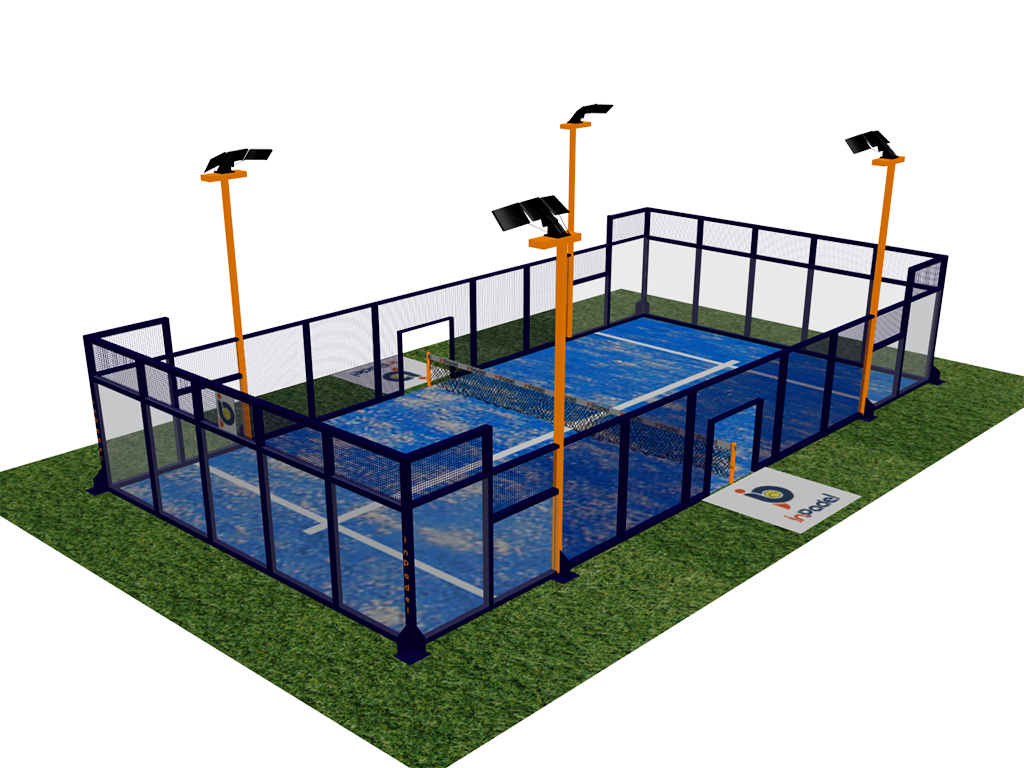
\includegraphics[width=\linewidth]{./DATA/images/intro/PaddleTennis_Court.png}\\
{\scriptsize\itshape Standard paddle tennis court with glass walls.}
\end{column}
\end{columns}
\end{frame}

% --- The Bandeja shot ----------------------------------------------------------
\begin{frame}{Why the \emph{bandeja} shot?}
\begin{columns}[T,onlytextwidth]
\begin{column}{0.55\textwidth}
\begin{itemize}
    \item Defensive overhead shot used to maintain net control after a lob.
    \item Biomechanically rich: arm extension, wrist position, impact timing, footwork.
    \item Mastery is what \alert{separates intermediate from advanced} amateurs.
    \item Ideal first target for an automated quality-assessment system.
\end{itemize}
\vspace{6pt}
\begin{exampleblock}{Scope of this thesis}
A single shot (\emph{bandeja}), a single output (5-class quality score), one reproducible end-to-end pipeline.
\end{exampleblock}
\end{column}
\begin{column}{0.43\textwidth}
\centering
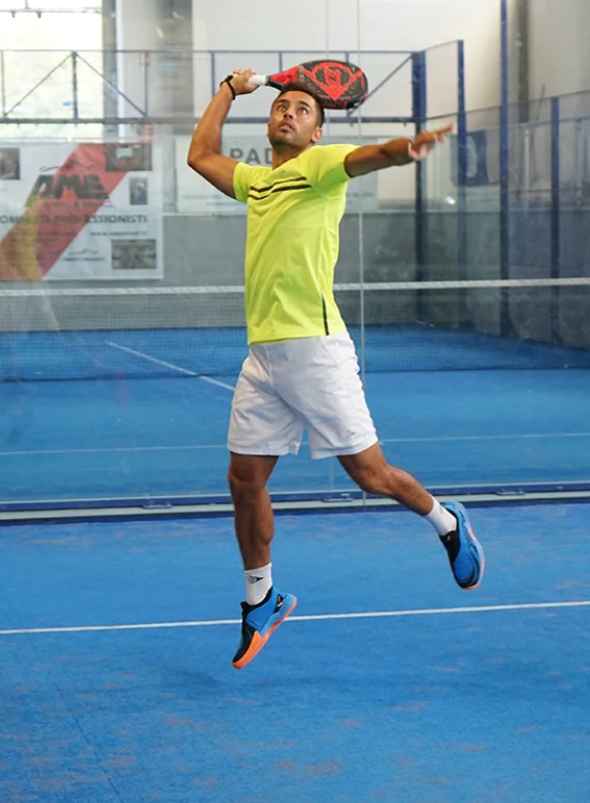
\includegraphics[width=0.95\linewidth]{./DATA/images/intro/Bandeja.png}\\
{\scriptsize\itshape The bandeja shot.}
\end{column}
\end{columns}
\end{frame}

% --- Hypothesis & Research Questions ------------------------------------------
\begin{frame}{Hypothesis \& Research Questions}
\begin{block}{Hypothesis}
\small A supervised \alert{recurrent model}, trained on pose-estimation data from \emph{bandeja} videos, can assign quality scores that are \alert{consistent with expert assessments} under controlled conditions.
\end{block}
\vspace{4pt}
\textbf{\color{tecdark}Research Questions:}
\begin{enumerate}\small
    \item How accurately does pose estimation extract key joints across skill levels?
    \item How well does the LSTM replicate expert-assigned scores, and with what deviation?
    \item To what extent does the model generalize to unseen performances?
    \item Is the learned representation specific to the \emph{bandeja}, or extensible to other shots?
\end{enumerate}
\end{frame}

% --- Contributions ------------------------------------------------------------
\begin{frame}{Contributions}
\begin{enumerate}\small
    \item A novel \alert{pose-based dataset} for paddle tennis: 484 \emph{bandeja} clips from 6 players, expert-graded (1--10) and mapped to 5 quality classes.
    \item Comparative evaluation of three temporal models -- \alert{BiLSTM, BiGRU, TCN} -- under identical pipeline, dataset, and metrics.
    \item Two sensitivity analyses (loss/optimizer grid and 5-point split sweep) that quantify how the system reacts to design choices.
    \item A fully \alert{reproducible end-to-end pipeline} (video $\rightarrow$ pose $\rightarrow$ sequence $\rightarrow$ classification) released as open-source code.
    \item Public release of the labeled dataset (2D joint trajectories + grades + metadata) as a benchmark for racket-sport motion analysis.
\end{enumerate}
\vspace{2pt}
\begin{infoBox}\small
Code: \url{https://github.com/CesarEmilioC/thesisRepo_A00830006}
\end{infoBox}
\end{frame}

% =============================================================================
%  Section 2 -- Methodology
% =============================================================================

\section{Methodology}

% --- Section divider --------------------------------------------------------
\sectiondivider{Methodology}{From raw video to a 5-class quality score}{sec:methodology}

% --- Subsection: Pipeline ---------------------------------------------------
\subsection{Pipeline}

\begin{frame}{End-to-end pipeline}
\hypertarget{sub:pipeline}{}%
\centering
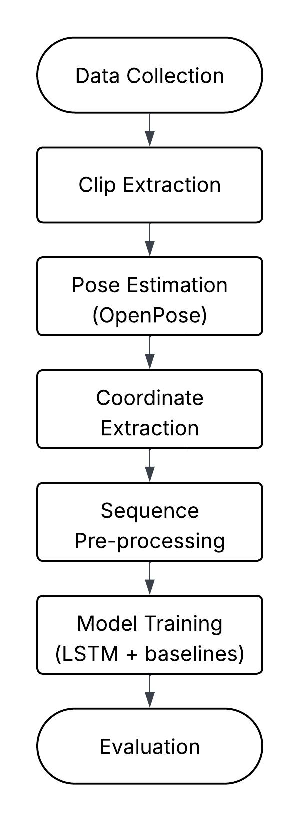
\includegraphics[width=0.92\linewidth,height=0.7\textheight,keepaspectratio]{./DATA/images/methodology/methodologyPipeline.pdf}\\[2pt]
{\scriptsize\itshape Seven modular stages, each independently inspectable and replaceable.}
\end{frame}

% --- Subsection: Data -------------------------------------------------------
\subsection{Data Collection \& Dataset}

\begin{frame}{Data collection \& labeling}
\hypertarget{sub:dataset}{}%
\begin{columns}[T,onlytextwidth]
\begin{column}{0.50\textwidth}
\textbf{\color{tecdark}Acquisition (controlled):}
\begin{itemize}\small
    \item iPhone 13, fixed \alert{vertical orientation}, 1080$\times$1920 HD @ 30 frames per second (FPS).
    \item 6 players, skill range: 6th category $\rightarrow$ professional.
    \item 484 clips, \alert{exactly 3\,s} each (90 frames @ 30\,\acrshort{FPS}).
\end{itemize}
\vspace{4pt}
\textbf{\color{tecdark}Labeling protocol:}
\begin{itemize}\small
    \item Each clip graded \alert{1--10} by a single expert coach.
    \item Grade embedded in filename (\texttt{\_grade}).
    \item Two evaluators: K.~Garc\'ia (CO), S.~Fasciolo (AR).
\end{itemize}
\end{column}
\begin{column}{0.48\textwidth}
\centering
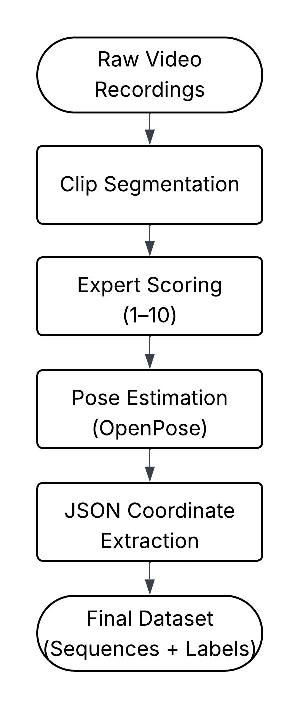
\includegraphics[width=\linewidth,height=0.68\textheight,keepaspectratio]{./DATA/images/methodology/dataCollection_Pipeline.pdf}\\[2pt]
{\scriptsize\itshape Six-stage data \& labeling workflow.}
\end{column}
\end{columns}
\end{frame}

\begin{frame}{Dataset \& 5-class mapping}
\begin{columns}[T,onlytextwidth]
\begin{column}{0.52\textwidth}
\small
Raw grades (1--10) $\rightarrow$ 5 quality classes:
\[
c = \min\!\bigl(\lfloor(y-1)/2\rfloor,\,4\bigr)
\]
\begin{center}\scriptsize
\begin{tabular}{lcc}
\toprule
\textbf{Class} & \textbf{Grades} & \textbf{N} \\
\midrule
Very Low  & 1--2  & 40  \\
Low       & 3--4  & 74  \\
Medium    & 5--6  & 132 \\
High      & 7--8  & 175 \\
Excellent & 9--10 & 63  \\
\midrule
\textbf{Total} & & \textbf{484} \\
\bottomrule
\end{tabular}
\end{center}
\vspace{2pt}
\begin{infoBox}\scriptsize
Skewed toward Medium / High $\rightarrow$ \alert{balanced class weights} in training.
\end{infoBox}
\end{column}
\begin{column}{0.46\textwidth}
\centering
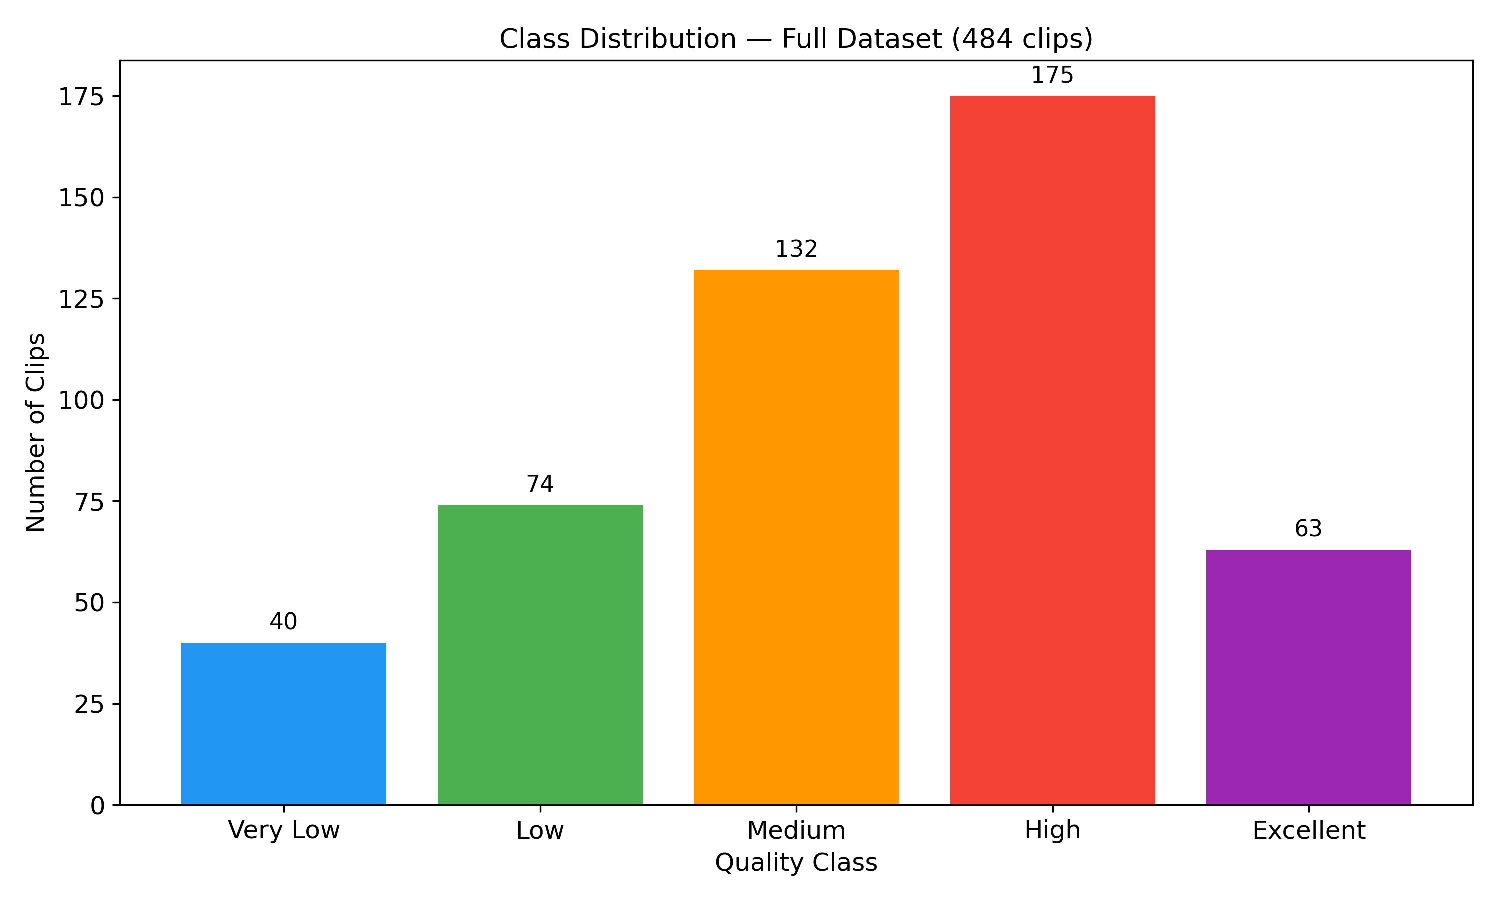
\includegraphics[width=\linewidth,height=0.62\textheight,keepaspectratio]{./DATA/images/experimentation/label_distribution.pdf}\\[2pt]
{\scriptsize\itshape Class distribution after the grade-to-class mapping.}
\end{column}
\end{columns}
\end{frame}

\begin{frame}{Dataset mosaic -- one frame per quality class}
\centering
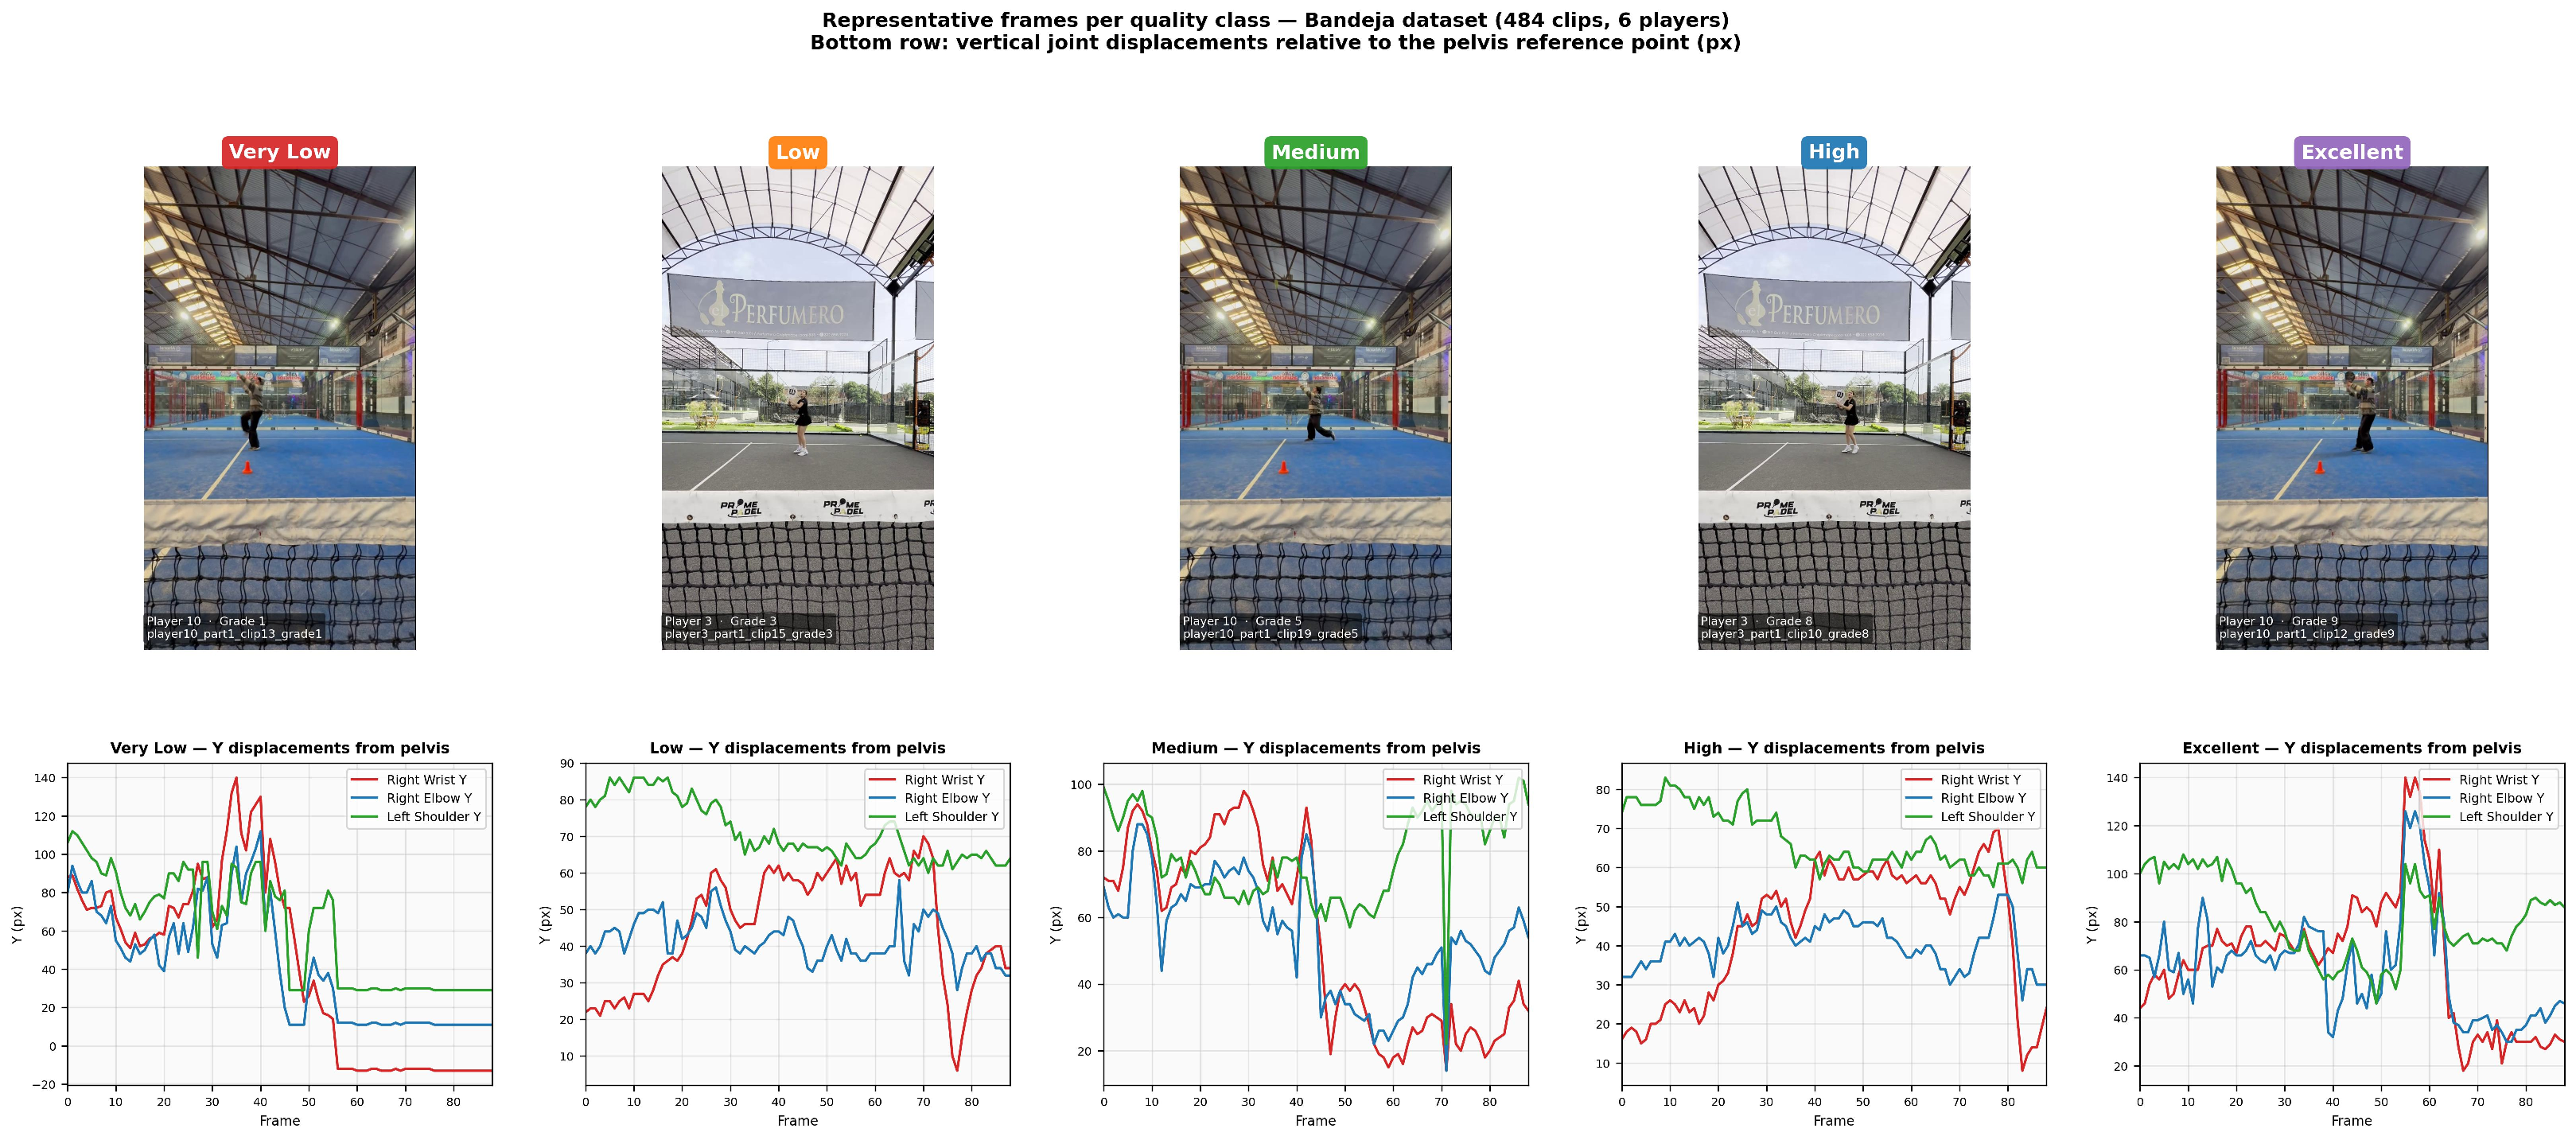
\includegraphics[width=\linewidth,height=0.66\textheight,keepaspectratio]{./DATA/images/experimentation/dataset_mosaic.pdf}\\[4pt]
{\footnotesize\textbf{\color{tecdark}Watch a representative clip:}}\\[1pt]
{\footnotesize
\setlength{\tabcolsep}{5pt}
\begin{tabular}{ccccc}
\href{https://github.com/CesarEmilioC/thesisRepo_A00830006/blob/main/Samples/mosaicSamples/player10_part1_clip13_grade1.mp4}{\textcolor{tecaccent}{\textbf{Very Low}}} &
\href{https://github.com/CesarEmilioC/thesisRepo_A00830006/blob/main/Samples/mosaicSamples/player3_part1_clip15_grade3.mp4}{\textcolor{tecorange}{\textbf{Low}}} &
\href{https://github.com/CesarEmilioC/thesisRepo_A00830006/blob/main/Samples/mosaicSamples/player10_part1_clip19_grade5.mp4}{\textcolor{tecblue}{\textbf{Medium}}} &
\href{https://github.com/CesarEmilioC/thesisRepo_A00830006/blob/main/Samples/mosaicSamples/player3_part1_clip10_grade8.mp4}{\textcolor{tecblue!70!tecgreen}{\textbf{High}}} &
\href{https://github.com/CesarEmilioC/thesisRepo_A00830006/blob/main/Samples/mosaicSamples/player10_part1_clip12_grade9.mp4}{\textcolor{tecgreen}{\textbf{Excellent}}}\\
{\scriptsize grades 1--2} & {\scriptsize grades 3--4} & {\scriptsize grades 5--6} & {\scriptsize grades 7--8} & {\scriptsize grades 9--10}\\
\end{tabular}
}\\[2pt]
{\scriptsize\itshape Click each class to open the corresponding clip on GitHub.}
\end{frame}

% --- Subsection: Pose features ---------------------------------------------
\subsection{Pose Features}

\begin{frame}{Pose estimation with OpenPose}
\hypertarget{sub:pose}{}%
\begin{columns}[T,onlytextwidth]
\begin{column}{0.52\textwidth}
\textbf{\color{tecdark}Joints retained (4)~\cite{Cao2019OpenPose}:}
\begin{itemize}\small
    \item \alert{Pelvis} -- positional reference (absolute).
    \item \alert{Left shoulder} -- trunk rotation.
    \item \alert{Right elbow} -- arm preparation.
    \item \alert{Right wrist} -- racket trajectory.
\end{itemize}
\vspace{4pt}
\textbf{\color{tecdark}Per clip $\Rightarrow$} sequence $\mathbf{X}_n\!\in\!\mathbb{R}^{F_n\times 8}$,\\
relative-to-pelvis $(x,y)$ for the 3 upper-body joints.
\vspace{4pt}
\begin{noteBox}\scriptsize
Linear interpolation fills missing detections.\\
Mean interpolation rate: \textbf{11.6\%} (consistent across classes).
\end{noteBox}
\end{column}
\begin{column}{0.46\textwidth}
\centering
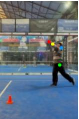
\includegraphics[width=\linewidth,height=0.65\textheight,keepaspectratio]{./DATA/images/methodology/poseEstimation_Example.pdf}\\[2pt]
{\scriptsize\itshape Pelvis (green), shoulder (blue), elbow (yellow), wrist (red)~\cite{Cao2019OpenPose}.}
\end{column}
\end{columns}
\end{frame}

\begin{frame}{What the model sees: \texttt{(90,\,8)} tensor of joint coordinates}
\hypertarget{sub:input}{}%
\begin{columns}[T,onlytextwidth]

% ---- LEFT: literal tensor preview ------------------------------------------
\begin{column}{0.54\textwidth}
\textbf{\color{tecdark}The literal input -- one tensor of shape \texttt{(90,\,8)} per clip:}\\[1pt]
{\scriptsize z-scored per clip $\cdot$ illustrative values $\cdot$ \textbf{720} numbers total}

\vspace{3pt}
\setlength{\tabcolsep}{2.5pt}
\renewcommand{\arraystretch}{1.02}
{\ttfamily\scriptsize
\begin{tabular}{r|rrrrrrrr}
\textbf{f} & \textbf{p$_x$} & \textbf{p$_y$} & \textbf{s$_x$} & \textbf{s$_y$} & \textbf{e$_x$} & \textbf{e$_y$} & \textbf{w$_x$} & \textbf{w$_y$}\\
\hline
0  & $-$1.20 & $-$0.85 & $-$0.42 &    0.13 & $-$0.78 &    0.24 & $-$1.05 &    0.31\\
1  & $-$1.15 & $-$0.81 & $-$0.38 &    0.17 & $-$0.70 &    0.30 & $-$0.95 &    0.40\\
2  & $-$1.10 & $-$0.78 & $-$0.34 &    0.21 & $-$0.62 &    0.36 & $-$0.85 &    0.49\\
\multicolumn{9}{c}{$\vdots$ \scriptsize (frames 3--43)}\\
44 &    0.05 & $-$0.12 &    0.28 &    0.95 &    0.55 &    1.62 &    1.10 &    2.18\\
45 &    0.07 & $-$0.10 &    0.31 &    0.98 &    0.58 &    1.65 &    1.13 &    2.21\\
\multicolumn{9}{c}{$\vdots$ \scriptsize (frames 46--88)}\\
89 &    0.85 &    0.42 &    0.71 &    0.18 &    1.08 &    0.55 &    0.92 &    0.81\\
\end{tabular}
}

\vspace{4pt}
{\scriptsize\textbf{Column legend:} \texttt{p}\,=\,pelvis (absolute), \texttt{s}\,=\,L-shoulder, \texttt{e}\,=\,R-elbow, \texttt{w}\,=\,R-wrist; subscripts $_x,_y$ = horizontal/vertical. The three upper-body joints are relative to the pelvis.}

\vspace{3pt}
\begin{infoBox}\scriptsize
\textbf{The model sees all 8 columns jointly} (pelvis + shoulder + elbow + wrist) -- not just one. The plot on the right visualises a single column for intuition.
\end{infoBox}
\end{column}

% ---- RIGHT: supporting trajectory plot ------------------------------------
\begin{column}{0.44\textwidth}
\centering
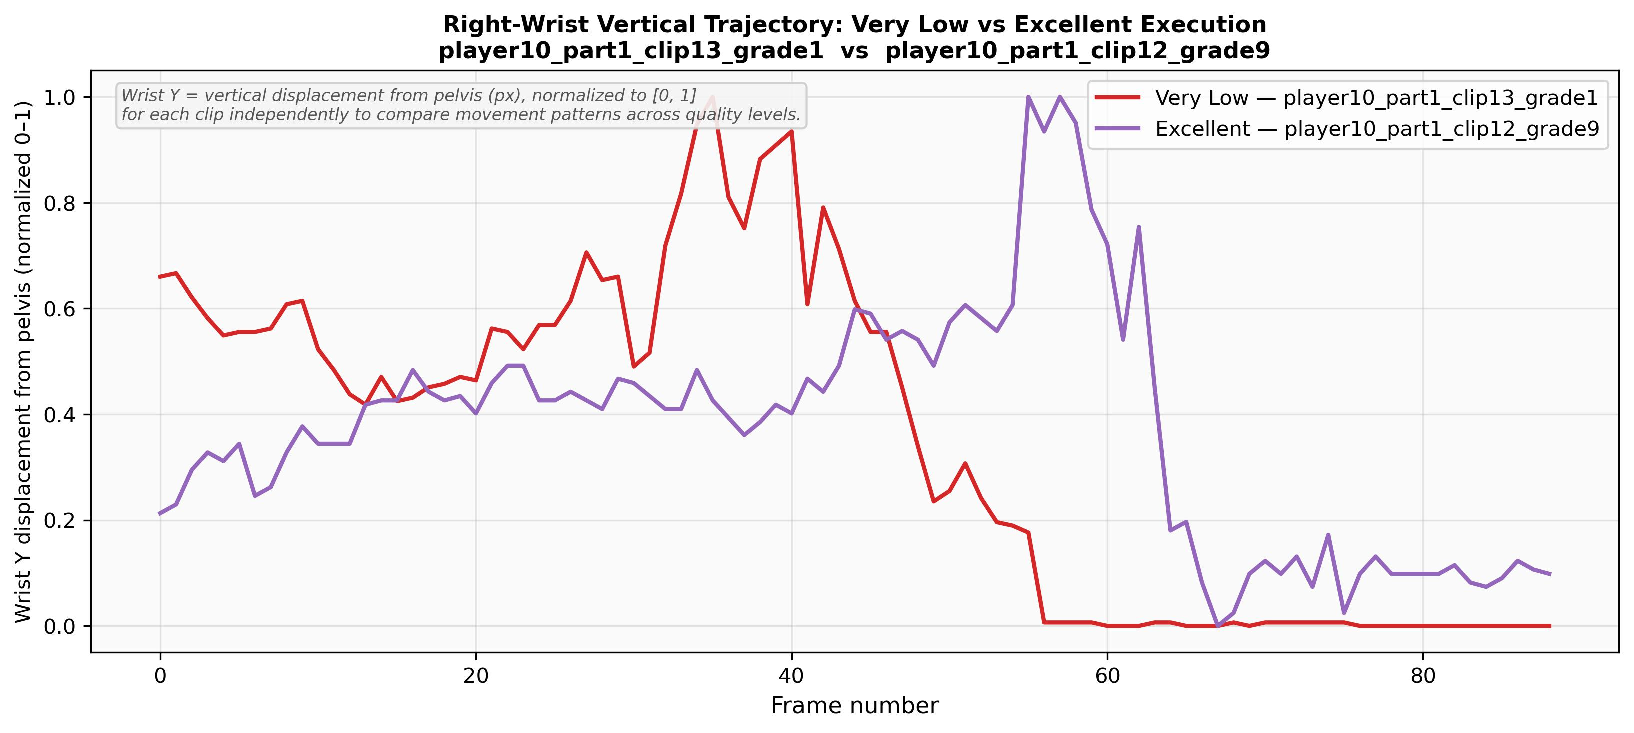
\includegraphics[width=\linewidth,height=0.56\textheight,keepaspectratio]{./DATA/images/methodology/trajectory_wrist_comparison.pdf}\\[2pt]
{\scriptsize\itshape \textbf{One of the 8 columns visualised:} the wrist trajectory across the 90 frames, for two clips of the same player. \alert{Excellent} (grade 9): smooth arc ($\sigma\!=\!40.1$~px). \alert{Very Low} (grade 1): irregular oscillations ($\sigma\!=\!184.1$~px). The remaining 7 columns evolve in parallel.}
\end{column}

\end{columns}
\end{frame}

% --- Subsection: Models -----------------------------------------------------
\subsection{Models}

\begin{frame}{Three temporal architectures}
\hypertarget{sub:models}{}%
\setlength{\tabcolsep}{4pt}
\small
\begin{center}
\begin{tabular}{l p{0.32\linewidth} p{0.36\linewidth}}
\toprule
\textbf{Model} & \textbf{Core block} & \textbf{Rationale} \\
\midrule
\textbf{BiLSTM}~\cite{Hochreiter1997LSTM} & 2 BiLSTM layers (64/32) + L2 weight decay + dropout 0.40/0.35 & 3-gate cell + cell state $\Rightarrow$ long-range memory \\
\addlinespace[2pt]
\textbf{BiGRU}~\cite{Cho2014GRU}  & 2 BiGRU layers (64/32) & 2-gate cell, fewer params (ablation) \\
\addlinespace[2pt]
\textbf{TCN}~\cite{Lea2017TCN}    & 3 dilated 1-D convs (kernel 3, dilation 1/2/4) + global average pooling (GAP) & Parallel processing, fixed receptive field \\
\bottomrule
\end{tabular}
\end{center}
\vspace{4pt}
\textbf{\color{tecdark}Shared training setup:}
\begin{itemize}\small
    \item Input $(90,8)$ $\rightarrow$ Softmax over 5 classes.
    \item Adam optimizer (Adaptive Moment estimation)~\cite{Adam2014}, sparse categorical cross-entropy, batch size 16, 100 epochs.
    \item EarlyStopping (patience 15), ReduceLROnPlateau, Gaussian noise augmentation (factor 2), \alert{balanced class weights}.
    \item 80/20 stratified split, seed 42.
\end{itemize}
\end{frame}

% --- Subsection: Evaluation -------------------------------------------------
\subsection{Evaluation Protocol}

\begin{frame}{Evaluation metrics -- categorical}
\hypertarget{sub:metrics}{}%
\small
For a $K$-class problem, with true positives ($\text{TP}_c$), false positives ($\text{FP}_c$), and false negatives ($\text{FN}_c$) per class $c$:
\vspace{4pt}
\begin{columns}[T,onlytextwidth]
\begin{column}{0.49\textwidth}
\begin{block}{Per-class\vphantom{Ag}}
\begin{minipage}[t][3.4cm][s]{\linewidth}
\centering\small
\vspace*{\fill}
$\displaystyle \text{Precision}_c = \frac{\text{TP}_c}{\text{TP}_c+\text{FP}_c}$\par
\vspace*{\fill}
$\displaystyle \text{Recall}_c = \frac{\text{TP}_c}{\text{TP}_c+\text{FN}_c}$\par
\vspace*{\fill}
$\displaystyle F_{1,c} = 2\cdot\frac{\text{Precision}_c \cdot \text{Recall}_c}{\text{Precision}_c + \text{Recall}_c}$\par
\vspace*{\fill}
\end{minipage}
\end{block}
\end{column}
\hspace{0.02\textwidth}
\begin{column}{0.49\textwidth}
\begin{block}{Aggregates\vphantom{Ag}}
\begin{minipage}[t][3.4cm][s]{\linewidth}
\centering\small
\vspace*{\fill}
$\displaystyle \text{Macro-}F_1 = \frac{1}{K}\sum_{c=1}^{K} F_{1,c}$\par
\vspace*{\fill}
$\displaystyle \text{Weighted-}F_1 = \sum_{c=1}^{K}\frac{n_c}{N}\,F_{1,c}$\par
\vspace*{\fill}
$\displaystyle \text{Accuracy} = \frac{\sum_c \text{TP}_c}{N}$\par
\vspace*{\fill}
\end{minipage}
\end{block}
\end{column}
\end{columns}
\vspace{4pt}
\begin{infoBox}\scriptsize
The \alert{confusion matrix} ($K\times K$) reveals \emph{where} errors land -- critical for ordinal tasks where adjacent-class confusion is expected but extreme-class confusion is not.
\end{infoBox}
\end{frame}

\begin{frame}{Evaluation metrics -- ordinal complement}
\begin{columns}[T,onlytextwidth]
\begin{column}{0.55\textwidth}
\small
The 5 quality classes carry a \alert{natural ordering}:
\[
\text{Very Low}\!<\!\text{Low}\!<\!\text{Medium}\!<\!\text{High}\!<\!\text{Excellent}
\]
Accuracy / F1 treat \emph{all} misclassifications as equally wrong. \alert{Spearman's $\rho$} captures monotonic agreement between predicted and true class rankings:
\[
\rho \;=\; \frac{\sum_i (R(y_i)\!-\!\overline{R(y)})\,(R(\hat{y}_i)\!-\!\overline{R(\hat{y})})}{\sqrt{\sum_i(R(y_i)\!-\!\overline{R(y)})^2 \sum_i(R(\hat{y}_i)\!-\!\overline{R(\hat{y})})^2}}
\]
\end{column}
\begin{column}{0.42\textwidth}
\begin{exampleblock}{Reading $\rho$}
\small
\begin{itemize}
    \item $\rho \!=\! +1$: perfect ordinal agreement.
    \item $\rho \!=\! 0$: no ordinal association.
    \item $\rho \!=\! -1$: perfect inverse ordering.
    \item Each $\rho$ paired with a $p$-value; \alert{$p\!<\!0.05$} required for statistical significance.
\end{itemize}
\end{exampleblock}
\vspace{4pt}
\begin{noteBox}\scriptsize
A high $\rho$ with modest accuracy means the model preserves the quality gradient even when the exact class is wrong.
\end{noteBox}
\end{column}
\end{columns}
\end{frame}

% =============================================================================
%  Section 3 -- Experimentation & Results
% =============================================================================

\section{Experimentation \& Results}

% --- Section divider --------------------------------------------------------
\sectiondivider{Experimentation \& Results}{Five experiments, two sensitivity sweeps, one headline finding}{sec:experiments}

% --- Subsection: LSTM Progression ------------------------------------------
\subsection{LSTM Evolution}

\begin{frame}{LSTM evolution: Stage 01 $\rightarrow$ Stage 02 $\rightarrow$ Stage 03}
\hypertarget{sub:evolution}{}%
\setlength{\tabcolsep}{3pt}
\renewcommand{\arraystretch}{0.95}
\footnotesize
\begin{center}
\textbf{Table 4.} \itshape BiLSTM stage progression on 80/20 stratified split (seed 42).\\[1pt]
\upshape
\begin{tabular}{l c c c}
\toprule
 & \textbf{Stage 01} & \textbf{Stage 02} & \textbf{Stage 03 (final)} \\
\midrule
\textbf{Dataset}        & 280 clips, 5 players & 484 clips, 6 players & 484 clips, 6 players \\
\textbf{Output classes} & 10 (raw grades)      & 5 (grouped)          & 5 (grouped) \\
\textbf{Joints / feats} & 3 / 6                & 4 / 8                & 4 / 8 \\
\textbf{Interpolation}  & --                   & linear               & linear \\
\textbf{Class weights}  & --                   & balanced             & balanced \\
\textbf{Hidden units}\textsuperscript{*}   & 128 / 64             & 128 / 64             & \alert{64 / 32} \\
\textbf{Regularization} & --                   & --                   & L2 ($10^{-4}$), dropout 0.40/0.35 \\
\textbf{Augmentation}   & --                   & --                   & Gaussian noise $\sigma\!=\!0.02$, $\times 2$ \\
\midrule
\textbf{Accuracy}       & 16.1\%               & 24.7\%               & \textbf{29.9\%} \\
\textbf{Macro F1}       & 0.09                 & 0.23                 & 0.23 \\
\bottomrule
\end{tabular}\\[2pt]
{\scriptsize\itshape \textsuperscript{*}All three stages use a \alert{2-layer stacked Bidirectional LSTM}; only the hidden-unit sizes per layer change.}
\end{center}
\vspace{2pt}
\begin{infoBox}\scriptsize
\textbf{Largest gain: $+8.6$ pp} came from \alert{pipeline changes} (5-class, interpolation, class weights), not from architecture. \textbf{\color{tecdark}Stage 03 is the documented final BiLSTM}; two sensitivity analyses push it further (next slides).
\end{infoBox}
\end{frame}

% --- Stage progression frame removed: redundant with the Table-3 frame above.
%     The diagnostic narrative (why each stage's interventions, what pain
%     each one fixed) is preserved in others/QA_BANK.md and the deep dive
%     for Q&A preparation, but does not need its own slide.

% --- Subsection: Model Comparison ------------------------------------------
\subsection{Model Comparison}

\begin{frame}{Comparison of three temporal models}
\hypertarget{sub:comparison}{}%
\setlength{\tabcolsep}{6pt}
\small
\begin{center}
\textbf{Table 5.} \itshape Head-to-head comparison of the three temporal architectures (80/20 split, seed 42).\\[2pt]
\upshape
\begin{tabular}{l c c c}
\toprule
\textbf{Metric} & \textbf{BiLSTM (Stage 03)} & \textbf{BiGRU (Stage 01)} & \textbf{TCN (Stage 01)} \\
\midrule
Architecture           & BiLSTM 64/32 & BiGRU 64/32 & 3$\times$ 1-D conv.\ (Conv1D) \\
Test set               & 97           & 97          & 97 \\
\midrule
\textbf{Accuracy}      & \textbf{29.9\%} & 26.8\%   & \textbf{29.9\%} \\
\textbf{Macro F1}      & 0.23         & 0.21        & \textbf{0.24} \\
\textbf{Weighted F1}   & \textbf{0.30} & 0.26       & \textbf{0.30} \\
Spearman $\rho$ ($p$)  & 0.03 (0.76)  & 0.12 (0.26) & 0.14 (0.18) \\
\bottomrule
\end{tabular}
\end{center}
\vspace{4pt}
\begin{itemize}\small
    \item BiLSTM and TCN tied on accuracy; TCN slightly higher macro F1 (better on \emph{Excellent}).
    \item BiGRU trails by 3.1~pp -- merged gating loses temporal information.
    \item Severe overfitting: BiLSTM and BiGRU reach train $\sim\!100\%$, TCN plateaus at $\sim\!80\%$; test $\sim\!30\%$ for all $\Rightarrow$ data bottleneck.
\end{itemize}
\end{frame}

\begin{frame}{Stage 03 BiLSTM: confusion matrix}
\begin{columns}[T,onlytextwidth]
\begin{column}{0.55\textwidth}
\centering
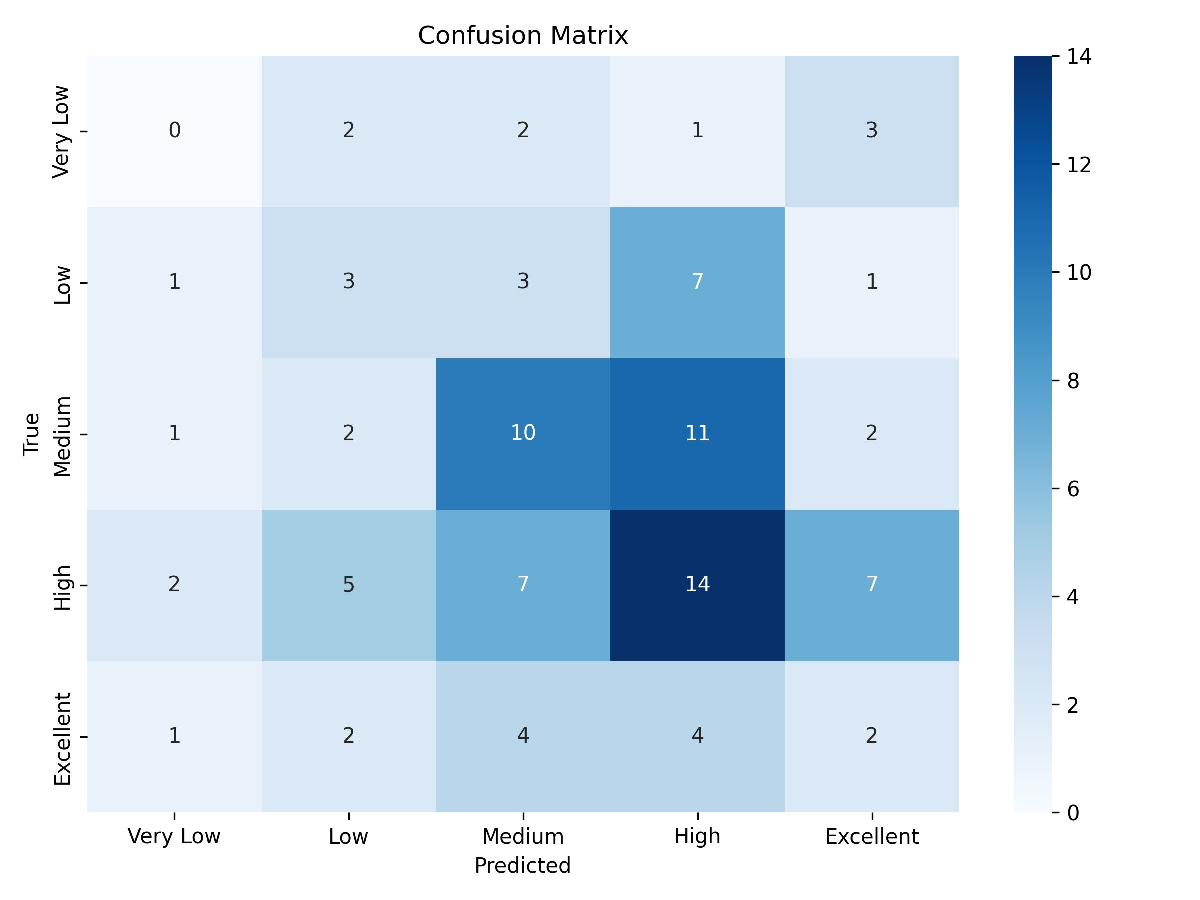
\includegraphics[width=\linewidth,height=0.72\textheight,keepaspectratio]{./DATA/images/experimentation/lstm_test03_confusion.pdf}\\[2pt]
{\scriptsize\textbf{Figure 9.} \itshape Stage 03 BiLSTM confusion matrix on the 80/20 test fold ($n\!=\!97$).}
\end{column}
\begin{column}{0.43\textwidth}\small
\textbf{\color{tecdark}Observations:}
\begin{itemize}
    \item Diagonal mass on \alert{Medium} (10/26) and \alert{High} (14/35).
    \item \emph{Very Low} (8 samples): zero recall -- spreads to Low / Medium.
    \item Off-diagonal mass on \alert{adjacent} classes $\Rightarrow$ ordinal confusion.
    \item No catastrophic Excellent$\leftrightarrow$Very Low confusion: the model has learned the gross gradient.
\end{itemize}
\end{column}
\end{columns}
\end{frame}

% --- Subsection: Sensitivity Analyses --------------------------------------
\subsection{Sensitivity Analyses}

\begin{frame}{Sensitivity 1: Loss function $\times$ Optimizer (BiLSTM)}
\hypertarget{sub:sensitivity}{}%
\begin{columns}[T,onlytextwidth]
\begin{column}{0.50\textwidth}
\setlength{\tabcolsep}{4pt}\scriptsize
\begin{center}
\textbf{Table 6.} \itshape Sensitivity 1 -- 2$\times$2 loss/optimizer grid.\\[2pt]
\upshape
\begin{tabular}{l l c c c}
\toprule
\textbf{Loss} & \textbf{Opt.} & \textbf{Acc.} & \textbf{F1$_m$} & \textbf{$\rho$ ($p$)} \\
\midrule
XEnt    & Adam (baseline) & 26.8\% & 0.21 & $-$0.02 (0.85) \\
\rowcolor{tecblue!10}
\textbf{XEnt} & \textbf{SGD}(0.9) & \textbf{35.1\%} & \textbf{0.30} & \textbf{0.19 (0.06)} \\
MSE     & Adam            & 35.1\% & 0.27 & 0.10 (0.31) \\
MSE     & SGD(0.9)        & 27.8\% & 0.23 & 0.07 (0.50) \\
\bottomrule
\end{tabular}
\end{center}
\vspace{4pt}
\textbf{\color{tecdark}Key findings:}
\begin{itemize}\scriptsize
    \item \alert{Cross-entropy (XEnt) + Stochastic Gradient Descent (SGD)}: $+8.3$~pp accuracy, $+0.09$ F1, $\rho\!=\!0.19$ ($p\!=\!0.06$) -- strongest single BiLSTM run.
    \item Adam~\cite{Adam2014} overfits faster on 484 clips; SGD's smoother updates win.
    \item Combining both changes (Mean Squared Error (MSE) + SGD) \emph{does not} stack.
\end{itemize}
\end{column}
\begin{column}{0.48\textwidth}
\centering
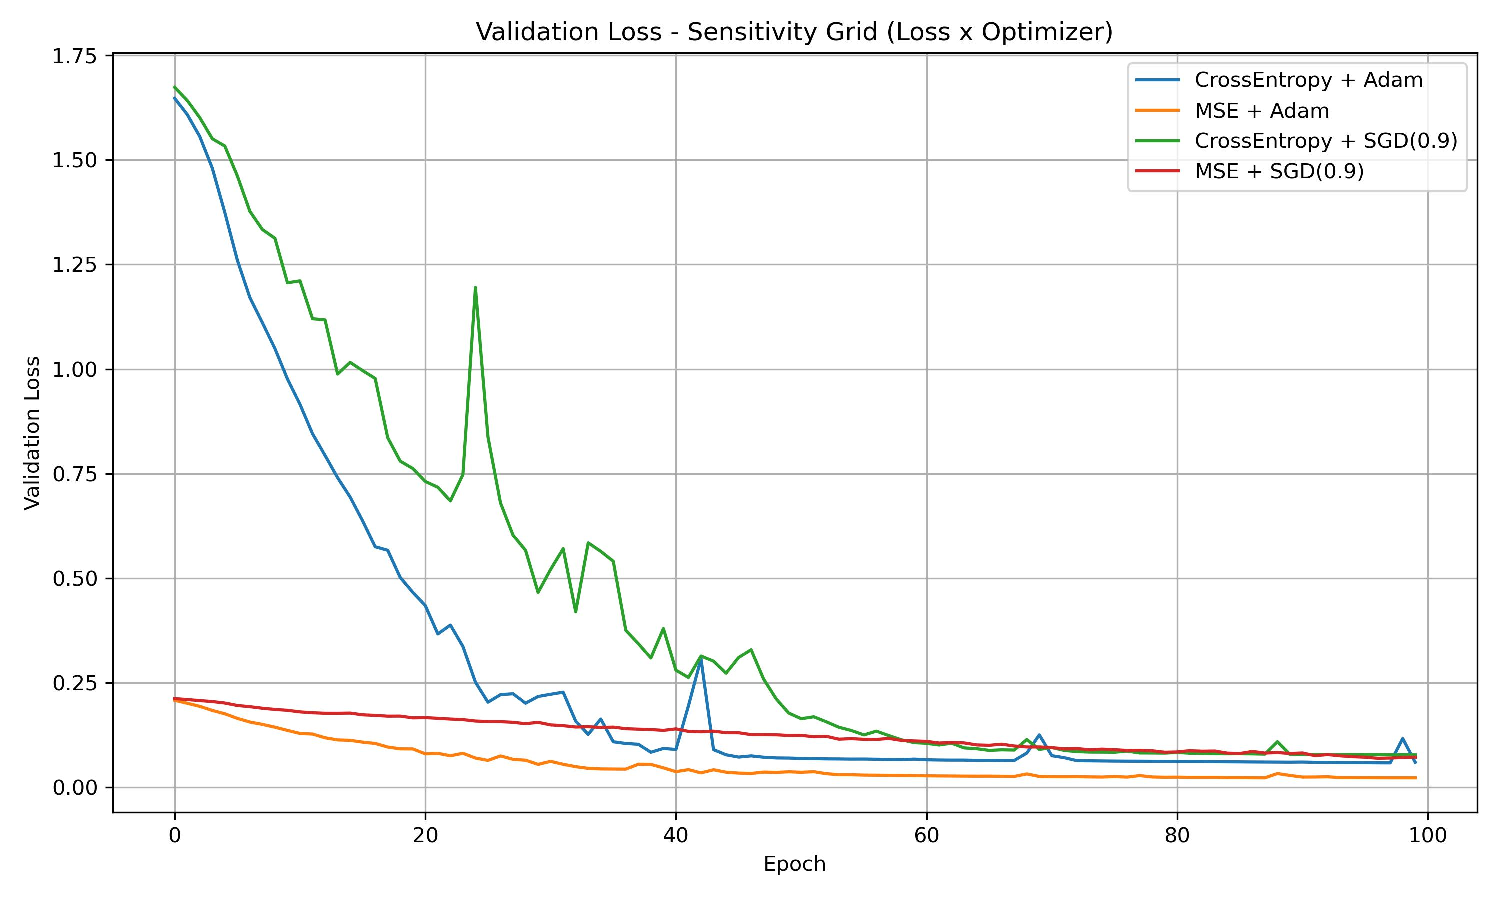
\includegraphics[width=\linewidth,height=0.7\textheight,keepaspectratio]{./DATA/images/experimentation/sensitivity_overlay.pdf}\\[2pt]
{\scriptsize\textbf{Figure 10.} \itshape Per-cell val-loss curves; MSE and XEnt sit on different numerical scales (not directly comparable). Ranking by test accuracy is in Table~6 -- winner: \alert{XEnt\,+\,SGD at 35.1\%}.}
\end{column}
\end{columns}
\end{frame}

\begin{frame}{Sensitivity 2: Train/Test split ratio (BiLSTM)}
\begin{columns}[T,onlytextwidth]
\begin{column}{0.50\textwidth}
\setlength{\tabcolsep}{4pt}\scriptsize
\begin{center}
\textbf{Table 7.} \itshape Sensitivity 2 -- 5-point train-fraction sweep.\\[2pt]
\upshape
\begin{tabular}{c c c c c}
\toprule
\textbf{Train frac.} & \textbf{Train / Test} & \textbf{Acc.} & \textbf{F1$_m$} & \textbf{$\rho$ ($p$)} \\
\midrule
0.50 & 242 / 242 & 35.5\% & 0.29 & \textbf{0.22 ($<\!0.001$)} \\
\rowcolor{tecblue!10}
\textbf{0.60} & 290 / 194 & \textbf{36.1\%} & 0.28 & \textbf{0.23 (0.001)} \\
0.70 & 338 / 146 & 34.2\% & 0.28 & 0.14 (0.09) \\
0.80\,(base)$^\dagger$ & 387 / 97 & \textbf{29.9\%} & 0.23 & 0.03 (0.76) \\
0.90 & 435 / 49  & 28.6\% & 0.24 & 0.05 (0.71) \\
\bottomrule
\end{tabular}\\[2pt]
{\tiny $^\dagger$The 0.80 row reports the documented Stage 03 final (LSTM Test03); the four other fractions come from the \texttt{runSplitAnalysis} sweep. Both share architecture, hyperparameters, and stratified split (\texttt{random\_state=42}); the $\sim$3\,pp run-to-run variance between code paths is consistent with non-explicit RNG seeding at $N\!=\!484$.}
\end{center}
\vspace{2pt}
\textbf{\color{tecdark}Counter-intuitive:}
\begin{itemize}\scriptsize
    \item Smaller training fractions \alert{win}.
    \item 0.60: \textbf{36.1\%}, $\rho\!=\!0.23$, $p\!=\!0.001$ -- the \emph{only} BiLSTM run with statistically significant $\rho$.
    \item Augmentation ($\times 2$) inflates training redundancy beyond what 100 epochs can absorb.
\end{itemize}
\end{column}
\begin{column}{0.48\textwidth}
\centering
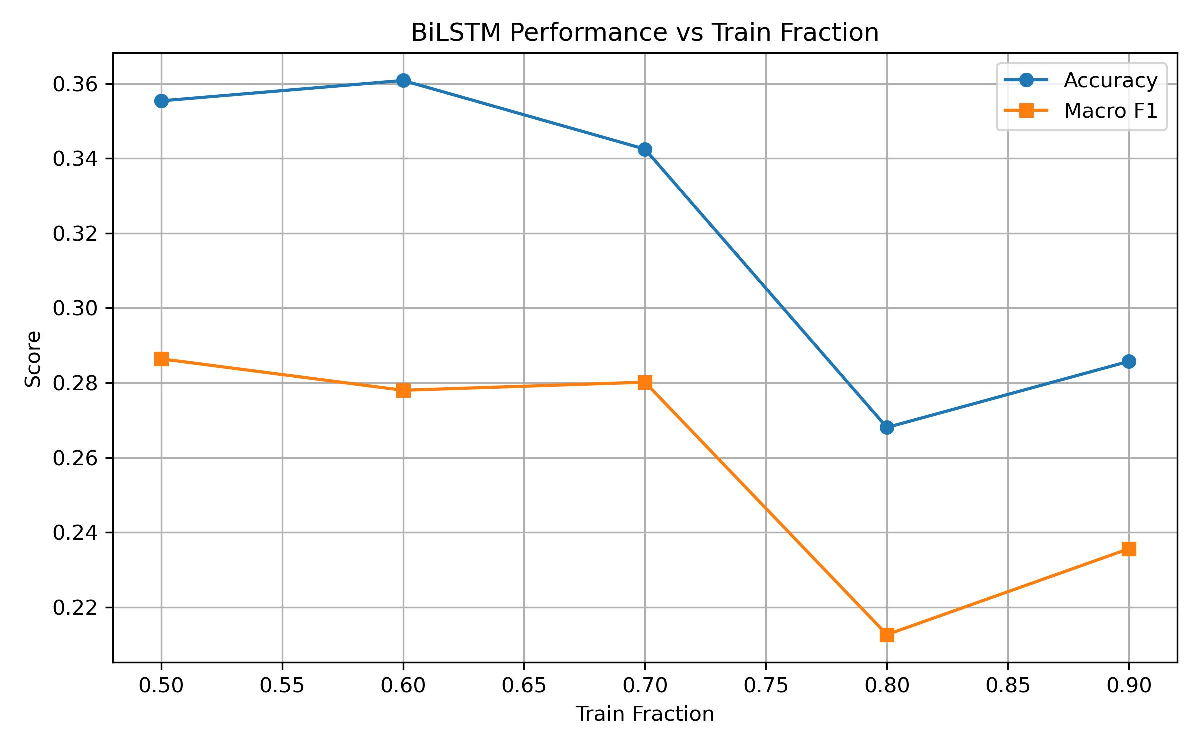
\includegraphics[width=\linewidth,height=0.7\textheight,keepaspectratio]{./DATA/images/experimentation/split_trend.pdf}\\[2pt]
{\scriptsize\textbf{Figure 11.} \itshape Accuracy and macro F1 vs.\ training fraction.}
\end{column}
\end{columns}
\end{frame}

% --- Subsection: Headline Finding ------------------------------------------
\subsection{Headline Finding}

\begin{frame}{\emph{Method is data-limited, not method-limited}}
\hypertarget{sub:headline}{}%
\begin{columns}[T,onlytextwidth]
\begin{column}{0.45\textwidth}
\centering
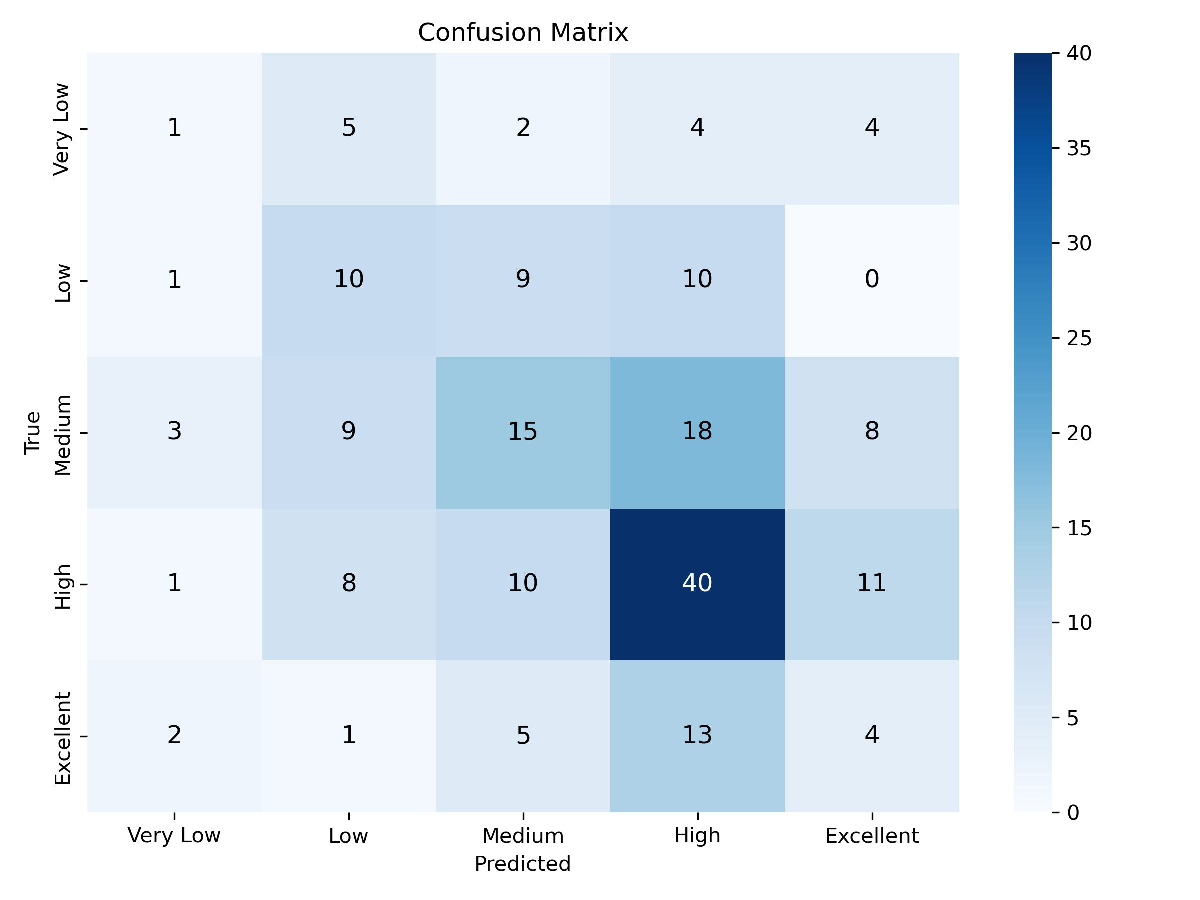
\includegraphics[width=\linewidth,height=0.66\textheight,keepaspectratio]{./DATA/images/experimentation/split_confusion_06.pdf}\\[2pt]
{\scriptsize\textbf{Figure 12.} \itshape Confusion matrix at the 60/40 split: broader coverage of minority classes.}
\end{column}
\hspace{0.02\textwidth}
\begin{column}{0.51\textwidth}
\begin{alertblock}{The $+6$ percentage-point (pp) gain -- and the $\rho$ flip}
\footnotesize Same architecture, same labels, same hyperparameters -- only the train/test fraction changed.\\[6pt]
\centerline{$29.9\%\;\Longrightarrow\;\textbf{36.1\%},\quad \rho\!:\;0.03\!\rightarrow\!\textbf{0.23},\quad p\!:\;0.76\!\rightarrow\!\textbf{0.001}$}\\[6pt]
{\scriptsize\itshape pp = percentage points: absolute difference between two percentages ($36.1-29.9=6.2$).}
\end{alertblock}
\vspace{4pt}
\begin{itemize}\scriptsize
    \item If the architecture / pipeline were the bottleneck, accuracy would be \alert{roughly flat across splits} -- ours is not.
    \item The Spearman $\rho$ \alert{crosses the conventional significance threshold} ($p\!<\!0.05$) only when the test fold is large enough -- the textbook signature of a \alert{data-limited regime}, not a methodological flaw.
\end{itemize}
\end{column}
\end{columns}
\end{frame}

% =============================================================================
%  Section 4 -- Conclusions & Future Work
% =============================================================================

\section{Conclusions \& Future Work}

% --- Section divider --------------------------------------------------------
\sectiondivider{Conclusions \& Future Work}{What works, what limits us, and where this goes next}{sec:conclusions}

% --- Subsection: Hypothesis -------------------------------------------------
\subsection{Hypothesis Verdict}

\begin{frame}[label=sub:verdict]{Hypothesis verdict: \emph{partial support}}
\begin{exampleblock}{Evidence in favor}
\small
\begin{itemize}
    \item End-to-end pipeline works (video $\rightarrow$ pose $\rightarrow$ sequence $\rightarrow$ 5-class score).
    \item All three architectures land \alert{well above the 20\% random baseline}.
    \item Confusion matrices show ordinal errors -- the gradient is being learned.
    \item Multi-split sweep: 60/40 reaches \textbf{36.1\%}, $\rho\!=\!0.23$ ($p\!=\!0.001$).
\end{itemize}
\end{exampleblock}
\begin{alertblock}{Evidence against full validation}
\small
\begin{itemize}
    \item Documented final model (Test03): 29.9\% -- not deployment-ready.
    \item Generalization gap: $\sim$70~pp between training and test accuracy.
    \item Spearman $\rho$ at 80/20 not significant ($p\!>\!0.05$).
\end{itemize}
\end{alertblock}
{\footnotesize\itshape Proof of concept: the method works at the present scale; closing the remaining gap is a data \& labeling problem.}
\end{frame}

% --- Subsection: Limitations ------------------------------------------------
\subsection{Limitations}

\begin{frame}[label=sub:limitations]{Limitations}
\begin{itemize}\small
    \item \textbf{Dataset size}: 484 clips across 6 players -- minority-class supports as low as 8 and 13 in the test set.
    \item \textbf{Single-evaluator labels}: no inter-rater reliability computed (no Cohen's $\kappa$ or Intraclass Correlation Coefficient, ICC).
    \item \textbf{2D, 4 joints, 8 features}: no joint angles, no angular velocities, no lower-body, no depth.
    \item \textbf{Player leakage}: stratified split mixes the same player across train and test (no Leave-One-Player-Out, LOPO, evaluation yet).
    \item \textbf{Recording setup}: single lateral smartphone view $\Rightarrow$ self-occlusion + motion blur $\Rightarrow$ 11.6\% interpolation rate.
    \item \textbf{Categorical loss}: cross-entropy ignores the ordinal structure of the 5 quality classes.
\end{itemize}
\end{frame}

% --- Subsection: Future Work ------------------------------------------------
\subsection{Future Work \& Scalability}

\begin{frame}[label=sub:future]{Future work -- four highest-priority actions}
\begin{enumerate}\small
    \item \textbf{Dataset expansion} to $\geq$ 1{,}000 clips, target $\geq$ 200 per class, more players and varied environments.
    \item \textbf{Validated labeling protocol}: dual-grading on $\geq$ 20\% of clips, Cohen's $\kappa$ / ICC, consensus resolution.
    \item \textbf{Richer features}: joint angles, angular velocities, lower-body, 3D pose (multi-camera).
    \item \textbf{LOPO cross-validation} across players to bound true generalization.
\end{enumerate}
\vspace{6pt}
\textbf{\color{tecdark}Model-side directions:}
\begin{itemize}\small
    \item Adopt the \alert{XEnt + SGD} configuration identified in Sensitivity~1.
    \item Reduce augmentation factor; strengthen L2 / dropout (per Sensitivity~2).
    \item Try ordinal-aware losses, attention on top of BiLSTM~\cite{Vaswani2017Attention}, or Spatio-Temporal Graph Convolutional Networks (ST-GCN)~\cite{Yan2018STGCN}.
    \item Add phase-level diagnostics $\rightarrow$ first step toward a true recommendation module.
\end{itemize}
\end{frame}

\begin{frame}{Scalability of the pipeline}
\begin{columns}[T,onlytextwidth]
\begin{column}{0.47\textwidth}
\textbf{\color{tecdark}Other paddle tennis shots}
\begin{itemize}\small
    \item v\'ibora, smash, volley, globo.
    \item Different joints / sequence lengths / quality rubrics.
\end{itemize}
\vspace{8pt}
\textbf{\color{tecdark}Other racket sports}
\begin{itemize}\small
    \item Tennis, squash, pickleball, badminton.
    \item Same infrastructure; sport-specific data \& labels.
\end{itemize}
\end{column}
\hspace{0.02\textwidth}
\begin{column}{0.47\textwidth}
\textbf{\color{tecdark}Beyond racket sports}
\begin{itemize}\small
    \item Team sports (multi-person pose).
    \item Gymnastics, martial arts (codified scoring).
    \item Physical rehabilitation, ergonomics.
    \item Dance, performing arts.
\end{itemize}
\vspace{8pt}
\begin{infoBox}\scriptsize
The bottleneck is \alert{not} the architecture -- it is the quality and quantity of labeled data.
\end{infoBox}
\end{column}
\end{columns}
\end{frame}

% --- Subsection: Demo & Resources ------------------------------------------
\subsection{Demo \& Resources}

\begin{frame}[label=sub:demo]{Live demo \& open resources}
\begin{exampleblock}{Interactive Colab demo (MODEL\_KEY selector)}
\small \texttt{final} (Test03) -- \texttt{best\_grid} (XEnt + SGD) -- \texttt{best\_split} (60/40)\\[2pt]
\href{https://drive.google.com/file/d/1ilXqfHP970POqXvRvfTO6ZWcD54KAfLP/view?usp=drive_link}{\color{tecaccent}\textbf{$\rightarrow$ Open the demo on Google Drive}}
\end{exampleblock}
\vspace{6pt}
\textbf{\color{tecdark}Open-source code \& artifacts:}
\begin{itemize}\small
    \item Repo: \url{https://github.com/CesarEmilioC/thesisRepo_A00830006}
    \item Command-Line Interface (CLI): \texttt{pose}, \texttt{trainLSTM/GRU/TCN}, \texttt{predict*}, \texttt{plot}, \texttt{animate}, \texttt{runSensitivity}, \texttt{runSplitAnalysis}.
    \item Saved weights: \texttt{lstmModel\_Sens\_C\_xent\_sgd\_27-04-2026.h5}, \texttt{lstmModel\_Split60\_27-04-2026.h5}, plus Test03.
    \item Output artifacts: training history JSON, learning curves, confusion matrices, classification reports, class-distribution plots.
\end{itemize}
\end{frame}

% --- Subsection: Acronyms --------------------------------------------------
\subsection{Acronyms}

% ---- Acronyms page 1: Models, layers, training -----------------------------
\begin{frame}{Acronyms -- models, layers \& training}
\setlength{\extrarowheight}{1pt}
\setlength{\tabcolsep}{4pt}
\footnotesize
\begin{columns}[T,onlytextwidth]
\begin{column}{0.48\textwidth}
\textbf{\color{tecdark}Recurrent \& sequence models}\\[2pt]
\begin{tabular}{@{}l@{\hspace{8pt}}p{0.66\linewidth}@{}}
\textbf{LSTM}    & Long Short-Term Memory \\
\textbf{BiLSTM}  & Bidirectional LSTM \\
\textbf{GRU}     & Gated Recurrent Unit \\
\textbf{BiGRU}   & Bidirectional GRU \\
\textbf{RNN}     & Recurrent Neural Network \\
\textbf{TCN}     & Temporal Convolutional Network \\
\textbf{CNN}     & Convolutional Neural Network \\
\textbf{Conv1D}  & one-dimensional convolutional layer \\
\textbf{ST-GCN}  & Spatio-Temporal Graph Convolutional Network \\
\textbf{GAP}     & Global Average Pooling \\
\textbf{PAF}     & Part Affinity Field (in OpenPose) \\
\textbf{BPTT}    & Backpropagation Through Time \\
\end{tabular}
\end{column}
\hspace{0.02\textwidth}
\begin{column}{0.48\textwidth}
\textbf{\color{tecdark}Optimizers, losses \& regularization}\\[2pt]
\begin{tabular}{@{}l@{\hspace{8pt}}p{0.66\linewidth}@{}}
\textbf{Adam}    & Adaptive Moment estimation (optimizer) \\
\textbf{SGD}     & Stochastic Gradient Descent (optimizer) \\
\textbf{XEnt}    & Cross-entropy (loss function) \\
\textbf{MSE}     & Mean Squared Error (loss function) \\
\textbf{L2}      & L2 weight regularization (ridge / weight decay) \\
\end{tabular}\\[10pt]
\textbf{\color{tecdark}Quality classes (1--10 $\to$ 5)}\\[2pt]
\begin{tabular}{@{}l@{\hspace{8pt}}l@{}}
\textbf{1--2}    & Very Low \\
\textbf{3--4}    & Low \\
\textbf{5--6}    & Medium \\
\textbf{7--8}    & High \\
\textbf{9--10}   & Excellent \\
\end{tabular}
\end{column}
\end{columns}
\end{frame}

% ---- Acronyms page 2: Evaluation, statistics, tooling ----------------------
\begin{frame}{Acronyms -- evaluation, statistics \& tooling}
\setlength{\extrarowheight}{1pt}
\setlength{\tabcolsep}{4pt}
\footnotesize
\begin{columns}[T,onlytextwidth]
\begin{column}{0.48\textwidth}
\textbf{\color{tecdark}Evaluation \& statistics}\\[2pt]
\begin{tabular}{@{}l@{\hspace{8pt}}p{0.66\linewidth}@{}}
\textbf{TP}      & True Positive \\
\textbf{FP}      & False Positive \\
\textbf{FN}      & False Negative \\
\textbf{TN}      & True Negative \\
\textbf{F1}      & F1-score (harmonic mean of precision and recall) \\
\textbf{F1$_m$}  & Macro F1 (unweighted mean of per-class F1) \\
\textbf{$\rho$}  & Spearman's rank correlation coefficient \\
\textbf{$\kappa$}& Cohen's kappa (inter-rater agreement) \\
\textbf{ICC}     & Intraclass Correlation Coefficient \\
\textbf{pp}      & percentage points (absolute, not relative) \\
\textbf{LOPO}    & Leave-One-Player-Out (cross-validation) \\
\textbf{ROC}     & Receiver Operating Characteristic \\
\textbf{DET}     & Detection Error Tradeoff \\
\end{tabular}
\end{column}
\hspace{0.02\textwidth}
\begin{column}{0.48\textwidth}
\textbf{\color{tecdark}Hardware, data \& tooling}\\[2pt]
\begin{tabular}{@{}l@{\hspace{8pt}}p{0.66\linewidth}@{}}
\textbf{FPS}     & Frames Per Second \\
\textbf{IMU}     & Inertial Measurement Unit \\
\textbf{JSON}    & JavaScript Object Notation \\
\textbf{CLI}     & Command-Line Interface \\
\textbf{GUI}     & Graphical User Interface \\
\textbf{GPU}     & Graphics Processing Unit \\
\textbf{API}     & Application Programming Interface \\
\end{tabular}\\[10pt]
\textbf{\color{tecdark}Reading the metrics}\\[2pt]
{\scriptsize
A model with accuracy $a$ and Spearman $\rho$ near zero can rank classes randomly; one with modest $a$ but high $\rho$ preserves the quality ordering even when the exact class is wrong -- the regime we target on an ordinal problem.}
\end{column}
\end{columns}
\end{frame}

% --- Subsection: Glossary --------------------------------------------------
\subsection{Glossary}

% ---- Glossary page 1: Sport & vision (6 entries) ---------------------------
\begin{frame}{Glossary -- sport \& vision}
\footnotesize
\begin{description}\setlength{\itemsep}{8pt}\setlength{\parsep}{0pt}
\item[\textbf{Amateur}]\hfill\\
A sport player who participates primarily for enjoyment, personal satisfaction, and skill development rather than for financial gain.

\item[\textbf{Bandeja}]\hfill\\
Paddle tennis stroke typically executed in response to a mid-height lob from the opponent. The ideal hitting zone is mid-court, at a height between a volley and a smash.

\item[\textbf{Paddle tennis} (padel)]\hfill\\
Racket sport that merges aspects of tennis and squash. Played primarily in doubles on an enclosed court roughly one-third the size of a tennis court, with playable walls integral to the game.

\item[\textbf{Biomechanics}]\hfill\\
Study of the mechanical laws governing the movement and structure of living organisms; here, the analysis of joint trajectories, forces, and timing that characterize human motion in sports.

\item[\textbf{Pose estimation}]\hfill\\
Computer vision technique that detects and tracks human body key-points (e.g., joints) from images or videos to estimate spatial positions and orientations.

\item[\textbf{OpenPose}]\hfill\\
Open-source real-time multi-person 2D pose-estimation framework that predicts body, hand, facial, and foot key-points using confidence maps and Part Affinity Fields.
\end{description}
\end{frame}

% ---- Glossary page 2: Data & training-time concepts (5 entries) ------------
\begin{frame}{Glossary -- data \& training-time concepts}
\footnotesize
\begin{description}\setlength{\itemsep}{8pt}\setlength{\parsep}{0pt}
\item[\textbf{Stratified split}]\hfill\\
Partition of a dataset into training and test subsets that preserves the proportion of samples per class within each subset -- used here to keep the five quality classes balanced across both splits.

\item[\textbf{Data augmentation}]\hfill\\
Synthesizing additional training samples from existing ones by applying small perturbations (e.g., Gaussian noise on coordinate trajectories) to enlarge the effective training set and improve generalization on small datasets.

\item[\textbf{Cross-entropy loss}]\hfill\\
Standard classification loss that compares the predicted probability distribution against the one-hot encoded true label. Penalizes confident wrong predictions more strongly than uncertain ones.

\item[\textbf{Dropout}]\hfill\\
Regularization that randomly disables a fraction of neurons during each training step, forcing the network not to rely on any single feature path. This thesis uses 0.40 and 0.35 in the two BiLSTM layers.

\item[\textbf{L2 regularization} (weight decay)]\hfill\\
Penalty added to the loss proportional to the squared magnitudes of the model weights. Pushes weights toward zero, smooths decision boundaries, and helps when training data is scarce.
\end{description}
\end{frame}

% ---- Glossary page 3: Evaluation & generalization concepts (6 entries) -----
\begin{frame}{Glossary -- evaluation \& generalization}
\footnotesize
\begin{description}\setlength{\itemsep}{7pt}\setlength{\parsep}{0pt}
\item[\textbf{Ordinal classification}]\hfill\\
Classification in which target classes follow a natural ordering (\textit{Very Low} $<$ \textit{Low} $<$ \textit{Medium} $<$ \textit{High} $<$ \textit{Excellent}). Adjacent-class errors are less wrong than distant-class errors, motivating rank-based metrics such as Spearman's $\rho$.

\item[\textbf{Confusion matrix}]\hfill\\
$K\!\times\!K$ matrix where entry $(i, j)$ records true-class-$i$ samples predicted as class $j$. Diagonal entries are correct; off-diagonal entries reveal where errors land.

\item[\textbf{Overfitting}]\hfill\\
A model fitting the training data very closely -- including noise and player-specific idiosyncrasies -- but failing to generalize. Visible here as a $\sim$70 pp gap between train and test accuracy.

\item[\textbf{Inter-rater reliability}]\hfill\\
Statistical agreement between two or more annotators evaluating the same content (e.g., Cohen's $\kappa$, ICC). Not computed in this thesis -- each clip was graded by one coach.

\item[\textbf{Leave-one-player-out} (LOPO)]\hfill\\
Cross-validation protocol in which all clips of one player are held out for testing per fold; gives a conservative estimate of generalization to truly unseen individuals.

\item[\textbf{Percentage points} (pp)]\hfill\\
Absolute difference between two percentages: $26.8\%\!\to\!36.1\%$ is a gain of $9.3$~pp, not a $35\%$ relative increase.
\end{description}
\end{frame}

% --- Subsection: References -------------------------------------------------
\subsection{References}

\begin{frame}[allowframebreaks]{References}
\scriptsize
\setlength{\bibitemsep}{3pt}
\setlength{\bibhang}{8pt}
\printbibliography[heading=none]
\end{frame}

% --- Closing slide (Q&A) ----------------------------------------------------
\begin{frame}[plain]
\centering
\vspace{0.8cm}
{\color{tecblue}\rule{0.7\linewidth}{1.2pt}}\\[14pt]
{\Huge\bfseries\color{tecdark}Thank you}\\[10pt]
{\large\color{slidegray}\itshape Questions \& discussion}\\[14pt]
{\color{tecblue}\rule{0.7\linewidth}{1.2pt}}\\[20pt]
{\small Cesar Emilio Casta\~no Marin \quad A00830006}\\
{\scriptsize Tecnol\'ogico de Monterrey -- MCC -- May 2026}\\[8pt]
{\scriptsize\url{https://github.com/CesarEmilioC/thesisRepo_A00830006}}
\end{frame}

% =============================================================================
%  Section 5 -- References (its own section, between Demo and Thank you)
% =============================================================================

\section{References}

\sectiondivider{References}{Works cited throughout the talk}{sec:references}

\begin{frame}[allowframebreaks]{References}
\scriptsize
\setlength{\bibitemsep}{3pt}
\setlength{\bibhang}{8pt}
\printbibliography[heading=none]
\end{frame}

% --- Closing slide (Q&A) ---------------------------------------------------
\begin{frame}[plain]
\centering
\vspace{0.8cm}
{\color{tecblue}\rule{0.7\linewidth}{1.2pt}}\\[14pt]
{\Huge\bfseries\color{tecdark}Thank you}\\[10pt]
{\large\color{slidegray}\itshape Questions \& discussion}\\[14pt]
{\color{tecblue}\rule{0.7\linewidth}{1.2pt}}\\[20pt]
{\small Cesar Emilio Casta\~no Marin \quad A00830006}\\
{\scriptsize Tecnol\'ogico de Monterrey -- MCC -- May 2026}\\[8pt]
{\scriptsize\url{https://github.com/CesarEmilioC/thesisRepo_A00830006}}
\end{frame}

% =============================================================================
%  Appendix -- back-matter shown AFTER the Thank-you slide.
%  Contains Acronyms and Glossary for committee reference.
% =============================================================================

\appendix

\section{Appendix}

\sectiondivider{Appendix}{Acronyms and glossary for reference}{sec:appendix}

% --- Subsection: Acronyms --------------------------------------------------
\subsection{Acronyms}

% ---- Acronyms page 1: Models, layers, training -----------------------------
\begin{frame}{Acronyms -- models, layers \& training}
\hypertarget{sub:appendix-acronyms}{}%
\setlength{\extrarowheight}{1pt}
\setlength{\tabcolsep}{4pt}
\footnotesize
\begin{columns}[T,onlytextwidth]
\begin{column}{0.48\textwidth}
\textbf{\color{tecdark}Recurrent \& sequence models}\\[2pt]
\begin{tabular}{@{}l@{\hspace{8pt}}p{0.66\linewidth}@{}}
\textbf{LSTM}    & Long Short-Term Memory \\
\textbf{BiLSTM}  & Bidirectional LSTM \\
\textbf{GRU}     & Gated Recurrent Unit \\
\textbf{BiGRU}   & Bidirectional GRU \\
\textbf{RNN}     & Recurrent Neural Network \\
\textbf{TCN}     & Temporal Convolutional Network \\
\textbf{CNN}     & Convolutional Neural Network \\
\textbf{Conv1D}  & one-dimensional convolutional layer \\
\textbf{ST-GCN}  & Spatio-Temporal Graph Convolutional Network \\
\textbf{GAP}     & Global Average Pooling \\
\textbf{PAF}     & Part Affinity Field (in OpenPose) \\
\textbf{BPTT}    & Backpropagation Through Time \\
\end{tabular}
\end{column}
\hspace{0.02\textwidth}
\begin{column}{0.48\textwidth}
\textbf{\color{tecdark}Optimizers, losses \& regularization}\\[2pt]
\begin{tabular}{@{}l@{\hspace{8pt}}p{0.66\linewidth}@{}}
\textbf{Adam}    & Adaptive Moment estimation (optimizer) \\
\textbf{SGD}     & Stochastic Gradient Descent (optimizer) \\
\textbf{XEnt}    & Cross-entropy (loss function) \\
\textbf{MSE}     & Mean Squared Error (loss function) \\
\textbf{L2}      & L2 weight regularization (ridge / weight decay) \\
\end{tabular}\\[10pt]
\textbf{\color{tecdark}Quality classes (1--10 $\to$ 5)}\\[2pt]
\begin{tabular}{@{}l@{\hspace{8pt}}l@{}}
\textbf{1--2}    & Very Low \\
\textbf{3--4}    & Low \\
\textbf{5--6}    & Medium \\
\textbf{7--8}    & High \\
\textbf{9--10}   & Excellent \\
\end{tabular}
\end{column}
\end{columns}
\end{frame}

% ---- Acronyms page 2: Evaluation, statistics, tooling ----------------------
\begin{frame}{Acronyms -- evaluation, statistics \& tooling}
\setlength{\extrarowheight}{1pt}
\setlength{\tabcolsep}{4pt}
\footnotesize
\begin{columns}[T,onlytextwidth]
\begin{column}{0.48\textwidth}
\textbf{\color{tecdark}Evaluation \& statistics}\\[2pt]
\begin{tabular}{@{}l@{\hspace{8pt}}p{0.66\linewidth}@{}}
\textbf{TP}      & True Positive \\
\textbf{FP}      & False Positive \\
\textbf{FN}      & False Negative \\
\textbf{TN}      & True Negative \\
\textbf{F1}      & F1-score (harmonic mean of precision and recall) \\
\textbf{F1$_m$}  & Macro F1 (unweighted mean of per-class F1) \\
\textbf{$\rho$}  & Spearman's rank correlation coefficient \\
\textbf{$\kappa$}& Cohen's kappa (inter-rater agreement) \\
\textbf{ICC}     & Intraclass Correlation Coefficient \\
\textbf{pp}      & percentage points (absolute, not relative) \\
\textbf{LOPO}    & Leave-One-Player-Out (cross-validation) \\
\textbf{ROC}     & Receiver Operating Characteristic \\
\textbf{DET}     & Detection Error Tradeoff \\
\end{tabular}
\end{column}
\hspace{0.02\textwidth}
\begin{column}{0.48\textwidth}
\textbf{\color{tecdark}Hardware, data \& tooling}\\[2pt]
\begin{tabular}{@{}l@{\hspace{8pt}}p{0.66\linewidth}@{}}
\textbf{FPS}     & Frames Per Second \\
\textbf{IMU}     & Inertial Measurement Unit \\
\textbf{JSON}    & JavaScript Object Notation \\
\textbf{CLI}     & Command-Line Interface \\
\textbf{GUI}     & Graphical User Interface \\
\textbf{GPU}     & Graphics Processing Unit \\
\textbf{API}     & Application Programming Interface \\
\end{tabular}\\[10pt]
\textbf{\color{tecdark}Reading the metrics}\\[2pt]
{\scriptsize
A model with accuracy $a$ and Spearman $\rho$ near zero can rank classes randomly; one with modest $a$ but high $\rho$ preserves the quality ordering even when the exact class is wrong -- the regime we target on an ordinal problem.}
\end{column}
\end{columns}
\end{frame}

% --- Subsection: Glossary --------------------------------------------------
\subsection{Glossary}

% ---- Glossary page 1: Sport & vision (6 entries) ---------------------------
\begin{frame}{Glossary -- sport \& vision}
\hypertarget{sub:appendix-glossary}{}%
\footnotesize
\begin{description}\setlength{\itemsep}{8pt}\setlength{\parsep}{0pt}
\item[\textbf{Amateur}]\hfill\\
A sport player who participates primarily for enjoyment, personal satisfaction, and skill development rather than for financial gain.

\item[\textbf{Bandeja}]\hfill\\
Paddle tennis stroke typically executed in response to a mid-height lob from the opponent. The ideal hitting zone is mid-court, at a height between a volley and a smash.

\item[\textbf{Paddle tennis} (padel)]\hfill\\
Racket sport that merges aspects of tennis and squash. Played primarily in doubles on an enclosed court roughly one-third the size of a tennis court, with playable walls integral to the game.

\item[\textbf{Biomechanics}]\hfill\\
Study of the mechanical laws governing the movement and structure of living organisms; here, the analysis of joint trajectories, forces, and timing that characterize human motion in sports.

\item[\textbf{Pose estimation}]\hfill\\
Computer vision technique that detects and tracks human body key-points (e.g., joints) from images or videos to estimate spatial positions and orientations.

\item[\textbf{OpenPose}]\hfill\\
Open-source real-time multi-person 2D pose-estimation framework that predicts body, hand, facial, and foot key-points using confidence maps and Part Affinity Fields.
\end{description}
\end{frame}

% ---- Glossary page 2: Data & training-time concepts (5 entries) ------------
\begin{frame}{Glossary -- data \& training-time concepts}
\footnotesize
\begin{description}\setlength{\itemsep}{8pt}\setlength{\parsep}{0pt}
\item[\textbf{Stratified split}]\hfill\\
Partition of a dataset into training and test subsets that preserves the proportion of samples per class within each subset -- used here to keep the five quality classes balanced across both splits.

\item[\textbf{Data augmentation}]\hfill\\
Synthesizing additional training samples from existing ones by applying small perturbations (e.g., Gaussian noise on coordinate trajectories) to enlarge the effective training set and improve generalization on small datasets.

\item[\textbf{Cross-entropy loss}]\hfill\\
Standard classification loss that compares the predicted probability distribution against the one-hot encoded true label. Penalizes confident wrong predictions more strongly than uncertain ones.

\item[\textbf{Dropout}]\hfill\\
Regularization that randomly disables a fraction of neurons during each training step, forcing the network not to rely on any single feature path. This thesis uses 0.40 and 0.35 in the two BiLSTM layers.

\item[\textbf{L2 regularization} (weight decay)]\hfill\\
Penalty added to the loss proportional to the squared magnitudes of the model weights. Pushes weights toward zero, smooths decision boundaries, and helps when training data is scarce.
\end{description}
\end{frame}

% ---- Glossary page 3: Evaluation & generalization concepts (6 entries) -----
\begin{frame}{Glossary -- evaluation \& generalization}
\footnotesize
\begin{description}\setlength{\itemsep}{7pt}\setlength{\parsep}{0pt}
\item[\textbf{Ordinal classification}]\hfill\\
Classification in which target classes follow a natural ordering (\textit{Very Low} $<$ \textit{Low} $<$ \textit{Medium} $<$ \textit{High} $<$ \textit{Excellent}). Adjacent-class errors are less wrong than distant-class errors, motivating rank-based metrics such as Spearman's $\rho$.

\item[\textbf{Confusion matrix}]\hfill\\
$K\!\times\!K$ matrix where entry $(i, j)$ records true-class-$i$ samples predicted as class $j$. Diagonal entries are correct; off-diagonal entries reveal where errors land.

\item[\textbf{Overfitting}]\hfill\\
A model fitting the training data very closely -- including noise and player-specific idiosyncrasies -- but failing to generalize. Visible here as a $\sim$70 pp gap between train and test accuracy.

\item[\textbf{Inter-rater reliability}]\hfill\\
Statistical agreement between two or more annotators evaluating the same content (e.g., Cohen's $\kappa$, ICC). Not computed in this thesis -- each clip was graded by one coach.

\item[\textbf{Leave-one-player-out} (LOPO)]\hfill\\
Cross-validation protocol in which all clips of one player are held out for testing per fold; gives a conservative estimate of generalization to truly unseen individuals.

\item[\textbf{Percentage points} (pp)]\hfill\\
Absolute difference between two percentages: $26.8\%\!\to\!36.1\%$ is a gain of $9.3$~pp, not a $35\%$ relative increase.
\end{description}
\end{frame}



\end{document}
